% Options for packages loaded elsewhere
\PassOptionsToPackage{unicode}{hyperref}
\PassOptionsToPackage{hyphens}{url}
\PassOptionsToPackage{dvipsnames,svgnames,x11names}{xcolor}
%
\documentclass[
  11pt,
]{article}
\usepackage{amsmath,amssymb}
\usepackage{setspace}
\usepackage{iftex}
\ifPDFTeX
  \usepackage[T1]{fontenc}
  \usepackage[utf8]{inputenc}
  \usepackage{textcomp} % provide euro and other symbols
\else % if luatex or xetex
  \usepackage{unicode-math} % this also loads fontspec
  \defaultfontfeatures{Scale=MatchLowercase}
  \defaultfontfeatures[\rmfamily]{Ligatures=TeX,Scale=1}
\fi
\ifPDFTeX\usepackage{lmodern}\fi
\ifPDFTeX\else
  % xetex/luatex font selection
  \setmainfont[]{TeX Gyre Termes}
  \setmathfont[]{DejaVu Math TeX Gyre}
\fi
% Use upquote if available, for straight quotes in verbatim environments
\IfFileExists{upquote.sty}{\usepackage{upquote}}{}
\IfFileExists{microtype.sty}{% use microtype if available
  \usepackage[]{microtype}
  \UseMicrotypeSet[protrusion]{basicmath} % disable protrusion for tt fonts
}{}
\makeatletter
\@ifundefined{KOMAClassName}{% if non-KOMA class
  \IfFileExists{parskip.sty}{%
    \usepackage{parskip}
  }{% else
    \setlength{\parindent}{0pt}
    \setlength{\parskip}{6pt plus 2pt minus 1pt}}
}{% if KOMA class
  \KOMAoptions{parskip=half}}
\makeatother
\usepackage{xcolor}
\usepackage[margin=2.2cm]{geometry}
\usepackage{longtable,booktabs,array}
\usepackage{calc} % for calculating minipage widths
% Correct order of tables after \paragraph or \subparagraph
\usepackage{etoolbox}
\makeatletter
\patchcmd\longtable{\par}{\if@noskipsec\mbox{}\fi\par}{}{}
\makeatother
% Allow footnotes in longtable head/foot
\IfFileExists{footnotehyper.sty}{\usepackage{footnotehyper}}{\usepackage{footnote}}
\makesavenoteenv{longtable}
\usepackage{graphicx}
\makeatletter
\def\maxwidth{\ifdim\Gin@nat@width>\linewidth\linewidth\else\Gin@nat@width\fi}
\def\maxheight{\ifdim\Gin@nat@height>\textheight\textheight\else\Gin@nat@height\fi}
\makeatother
% Scale images if necessary, so that they will not overflow the page
% margins by default, and it is still possible to overwrite the defaults
% using explicit options in \includegraphics[width, height, ...]{}
\setkeys{Gin}{width=\maxwidth,height=\maxheight,keepaspectratio}
% Set default figure placement to htbp
\makeatletter
\def\fps@figure{htbp}
\makeatother
\setlength{\emergencystretch}{3em} % prevent overfull lines
\providecommand{\tightlist}{%
  \setlength{\itemsep}{0pt}\setlength{\parskip}{0pt}}
\setcounter{secnumdepth}{-\maxdimen} % remove section numbering
\usepackage{float}\floatplacement{figure}{H}
\ifLuaTeX
  \usepackage{selnolig}  % disable illegal ligatures
\fi
\IfFileExists{bookmark.sty}{\usepackage{bookmark}}{\usepackage{hyperref}}
\IfFileExists{xurl.sty}{\usepackage{xurl}}{} % add URL line breaks if available
\urlstyle{same}
\hypersetup{
  pdftitle={Beyond the Approve/Reject Label: An Explainable, Fairness-Audited and Stability-Tested Machine Learning Framework for Credit Risk Assessment},
  pdfauthor={{[}Author 1 Name{]}, {[}Author 2 Name{]}, {[}Author 3 Name{]}; School of Computer Science and Engineering, Vellore Institute of Technology, Vellore, India; {[}email addresses{]}},
  colorlinks=true,
  linkcolor={black},
  filecolor={Maroon},
  citecolor={Blue},
  urlcolor={blue},
  pdfcreator={LaTeX via pandoc}}

\title{Beyond the Approve/Reject Label: An Explainable, Fairness-Audited
and Stability-Tested Machine Learning Framework for Credit Risk
Assessment}
\author{{[}Author 1 Name{]}, {[}Author 2 Name{]}, {[}Author 3
Name{]} \and School of Computer Science and Engineering, Vellore
Institute of Technology, Vellore, India \and {[}email addresses{]}}
\date{}

\begin{document}
\maketitle

\setstretch{1.1}
\hypertarget{abstract}{%
\section{Abstract}\label{abstract}}

Lenders increasingly rely on machine-learning (ML) models to estimate
the probability that a borrower will default, yet a model that returns
only ``approve'' or ``reject'' gives applicants, credit officers and
regulators little basis for trust, challenge or audit. This paper
presents an academic prototype that couples credit-risk prediction with
three supporting analyses: post-hoc explanation, group-fairness auditing
and prediction-stability testing. Using the Statlog German Credit
dataset (1,000 applicants, 30\% labelled as bad credit), we compare
logistic regression, random forest and XGBoost inside a leakage-free
preprocessing pipeline tuned by five-fold cross-validation. A random
forest was selected because its cross-validated ROC-AUC (0.792) was
within 0.01 of the best model (XGBoost, 0.797) while being the simpler
of the two ensembles. Because the dataset's documentation assigns five
times more cost to approving a bad borrower than to rejecting a good
one, the decision threshold was set to 0.27 using out-of-fold training
predictions. On a held-out test set of 200 applicants the model achieves
ROC-AUC 0.809, recall 0.850, precision 0.447, F1 0.586 and accuracy
0.640. SHAP values provide applicant-level and global explanations;
checking-account status, loan duration and savings were the most
influential features. A Fairlearn audit shows that applicants under 25
receive a markedly lower approval rate (23.1\%) than older applicants
(47.8\%), and that creditworthy women are wrongly rejected more often
than creditworthy men (51.2\% vs 42.4\%), even though sex is not a model
input. A perturbation test found that 96.5\% of test applicants kept the
same decision under ±5\% changes to loan amount and duration. The system
is delivered as a FastAPI service with a React dashboard. It is a
research prototype trained on small historical data, not a production
lending system, and its fairness findings are reported as identified
disparities rather than as evidence of a fair model.

\textbf{Keywords} --- credit risk assessment, explainable artificial
intelligence, SHAP, algorithmic fairness, Fairlearn, random forest,
cost-sensitive classification, prediction stability

\hypertarget{introduction}{%
\section{1. Introduction}\label{introduction}}

Credit risk assessment is the task of estimating how likely an applicant
is to fail to repay a loan. The estimate drives whether credit is
granted, how much is lent and at what price, so errors are costly in
both directions: approving applicants who later default produces direct
losses, while rejecting applicants who would have repaid denies them
access to finance and reduces the lender's business.

Historically, this judgement was made by loan officers following
institutional guidelines, later supported by statistical scorecards
built mainly on logistic regression. Scorecards remain popular precisely
because each variable's contribution to the score can be read off
directly. Over the last two decades, however, a large body of
benchmarking work has shown that ensemble learners such as random
forests and gradient boosting often rank applicants more accurately than
single statistical models {[}1{]}, {[}2{]}, {[}3{]}. Lending
institutions have accordingly moved towards these more flexible, but
less transparent, models.

This shift raises three concerns that predictive accuracy alone does not
address.

\begin{enumerate}
\def\labelenumi{\arabic{enumi}.}
\tightlist
\item
  \textbf{Explainability.} Ensemble models combine hundreds of decision
  trees, so the reason behind any single decision is not visible.
  Applicants refused credit, the officers who handle their cases and the
  supervisors who audit lenders all need to understand which factors
  drove a decision. Rudin argues that opaque models are especially
  problematic for high-stakes decisions {[}4{]}, and post-hoc tools such
  as LIME {[}5{]} and SHAP {[}6{]} have been developed partly in
  response.
\item
  \textbf{Fairness.} A model trained on historical lending outcomes can
  reproduce or amplify past disparities between demographic groups, even
  when protected attributes are removed, because other variables can act
  as proxies {[}7{]}, {[}8{]}. Empirical work on mortgage data has shown
  that more flexible ML models can change outcomes unevenly across
  groups {[}9{]}.
\item
  \textbf{Stability.} If a negligible change in an input, such as a
  slightly different loan amount, reverses a decision, then the decision
  is fragile and difficult to defend. Explanation methods themselves
  have also been shown to be sensitive to small perturbations {[}10{]},
  {[}11{]}.
\end{enumerate}

These concerns are usually studied separately: predictive benchmarks
focus on accuracy, explainability studies on interpretation, and
fairness studies on group metrics. This project brings them together in
a single, working prototype. For every applicant, the system reports a
risk prediction and probability, a SHAP-based explanation, and a
stability check; at the model level it reports evaluation metrics,
global feature importance and a group-fairness audit. All results in
this paper are produced by that implementation.

The remainder of the paper is organised as follows. Sections 2--4 state
the problem, objectives and research questions. Sections 5--6 review
related work and identify the gap addressed. Sections 7--14 describe the
dataset and methods, and Sections 15--16 the system. Sections 17--19
report and discuss results. Sections 20--23 cover limitations, current
progress, conclusions and future work.

\hypertarget{problem-statement}{%
\section{2. Problem Statement}\label{problem-statement}}

Given the attributes of a loan applicant, the system must estimate the
probability that the applicant will be a bad credit risk and convert
that estimate into a decision. The decision must be accompanied by (a)
an explanation of which applicant attributes increased or decreased the
estimated risk, (b) evidence on whether the model's decisions differ
systematically between demographic groups, and (c) evidence on whether
the decision changes under small, plausible variations of the
applicant's numeric inputs. The model must be evaluated with metrics
that reflect the unequal cost of the two kinds of error, rather than
with accuracy alone.

\hypertarget{research-objective}{%
\section{3. Research Objective}\label{research-objective}}

\textbf{Main objective.} To design, implement and evaluate a credit-risk
assessment framework in which every prediction is accompanied by an
interpretable explanation, the model's behaviour is audited across
demographic groups, and the robustness of individual decisions to small
input changes is measured.

The objective is broken into the following measurable sub-objectives:

\begin{itemize}
\tightlist
\item
  \textbf{O1 --- Prediction:} train and compare at least three
  classifiers using cross-validation and report accuracy, precision,
  recall, F1 and ROC-AUC on an untouched test set.
\item
  \textbf{O2 --- Cost-aware decisions:} derive a decision threshold from
  the dataset's asymmetric misclassification costs without using test
  data.
\item
  \textbf{O3 --- Explainability:} produce local (per-applicant) and
  global SHAP explanations expressed in terms of the original applicant
  attributes.
\item
  \textbf{O4 --- Fairness auditing:} measure approval rates, error
  rates, demographic parity difference and equalized odds difference for
  available sensitive attributes, and report sample-size limitations.
\item
  \textbf{O5 --- Stability:} quantify how often decisions change under
  small perturbations of non-sensitive numeric features, and identify
  the features to which decisions are most sensitive.
\item
  \textbf{O6 --- Integration:} expose all of the above through a
  documented REST API and an interactive web dashboard.
\end{itemize}

\hypertarget{research-questions}{%
\section{4. Research Questions}\label{research-questions}}

\begin{itemize}
\tightlist
\item
  \textbf{RQ1.} How well can standard ML classifiers rank and classify
  credit risk on the German Credit dataset, and how much does the choice
  of model matter?
\item
  \textbf{RQ2.} Which applicant attributes drive the selected model's
  predictions globally, and can SHAP values give consistent,
  human-readable explanations for individual decisions?
\item
  \textbf{RQ3.} Do the model's decisions differ across age, sex and
  foreign-worker groups, and how reliable are such measurements on a
  dataset of this size?
\item
  \textbf{RQ4.} How stable are individual decisions when loan amount and
  duration are perturbed slightly, and which features are most likely to
  flip a decision?
\item
  \textbf{RQ5.} Can prediction, explanation, fairness auditing and
  stability testing be integrated into a single practical system without
  compromising the evaluation protocol?
\end{itemize}

\hypertarget{related-work}{%
\section{5. Related Work}\label{related-work}}

\hypertarget{machine-learning-for-credit-scoring}{%
\subsection{5.1 Machine learning for credit
scoring}\label{machine-learning-for-credit-scoring}}

Baesens et al.~{[}1{]} compared a wide range of classifiers on eight
real credit datasets and found that several methods, including neural
networks and support vector machines, performed well, but that simple
logistic regression and linear discriminant analysis were often
competitive. More than a decade later, Lessmann et al.~{[}2{]} updated
this benchmark with 41 classifiers and several performance measures, and
reported that heterogeneous ensembles and random forests tended to
outperform the industry-standard logistic regression. Dastile et
al.~{[}3{]} systematically surveyed statistical and ML credit-scoring
studies from the preceding decade and found ensemble approaches to be
among the most frequently reported strong performers. The random forest
{[}12{]} and XGBoost {[}13{]} algorithms used in this work are among the
most widely applied ensemble methods in this literature.

\hypertarget{the-german-credit-dataset}{%
\subsection{5.2 The German Credit
dataset}\label{the-german-credit-dataset}}

The Statlog German Credit dataset donated by Hofmann {[}14{]} is one of
the most commonly used public credit datasets in ML research, partly
because it is small, complete and ships with a cost matrix. It is also
widely used in the fairness literature because it contains age, sex and
foreign-worker information; Kamiran and Calders, for example, used it to
evaluate pre-processing techniques for discrimination-aware
classification {[}15{]}. Grömping later documented serious coding errors
in the original attribute descriptions and released a corrected ``South
German Credit'' version {[}16{]}. We use the original data for
comparability with prior work and discuss the implications in Section
20.

\hypertarget{explainable-ai-in-credit-decisions}{%
\subsection{5.3 Explainable AI in credit
decisions}\label{explainable-ai-in-credit-decisions}}

Doshi-Velez and Kim {[}17{]} argue that interpretability should be
treated as a measurable property connected to concrete needs, such as
detecting bias or justifying decisions. Model-agnostic post-hoc methods
approximate a complex model's behaviour around a particular input: LIME
fits a local surrogate model {[}5{]}, while SHAP attributes a prediction
to features using Shapley values from cooperative game theory and
unifies several earlier attribution methods {[}6{]}. Lundberg et
al.~later developed an exact, polynomial-time algorithm for tree
ensembles (TreeSHAP) and showed how local explanations can be aggregated
into global insight {[}18{]}. In credit risk specifically, Bussmann et
al.~{[}19{]} combined gradient-boosted trees with Shapley values to
explain credit-risk predictions on peer-to-peer lending data, grouping
borrowers by the similarity of their explanations. In contrast, Rudin
{[}4{]} cautions that post-hoc explanations of black boxes can be
incomplete or misleading, and recommends inherently interpretable models
where they perform comparably.

\hypertarget{fairness-in-machine-learning-and-lending}{%
\subsection{5.4 Fairness in machine learning and
lending}\label{fairness-in-machine-learning-and-lending}}

Mehrabi et al.~{[}7{]} survey the sources of bias in ML systems and the
many definitions of fairness proposed to measure it. Two group-level
definitions are used in this work. Demographic parity compares the rate
of favourable decisions across groups, whereas equalized odds,
introduced by Hardt et al.~{[}20{]}, requires equal true-positive and
false-positive rates across groups. Kleinberg et al.~{[}21{]} and
Chouldechova {[}22{]} showed that, when base rates differ between
groups, calibration and equal error rates generally cannot be achieved
simultaneously, so any fairness assessment involves trade-offs and must
state which definition it uses. Barocas et al.~{[}8{]} discuss why
simply removing protected attributes (``fairness through unawareness'')
is insufficient. In credit markets, Fuster et al.~{[}9{]} found that
more flexible ML models increased predicted default-risk disparities
across racial and ethnic groups in US mortgage data. Fairlearn is an
open-source toolkit that implements group fairness metrics and
mitigation algorithms {[}23{]}, and is used in our audit.

\hypertarget{robustness-and-stability}{%
\subsection{5.5 Robustness and
stability}\label{robustness-and-stability}}

The adversarial-examples literature demonstrates that small, targeted
input changes can alter the output of an ML model {[}24{]}. For tabular
credit data, a related but more modest question is whether a decision is
stable under small, realistic variations of the applicant's numbers.
Alvarez-Melis and Jaakkola {[}10{]} showed that several interpretability
methods produce noticeably different explanations for nearly identical
inputs, and Slack et al.~{[}11{]} demonstrated that LIME and SHAP
explanations can be deliberately manipulated. These findings motivate
checking the stability of decisions alongside their explanations.

\hypertarget{research-gap}{%
\section{6. Research Gap}\label{research-gap}}

The reviewed work shows strong progress on each concern separately.
Large benchmarks {[}1{]}--{[}3{]} concentrate on predictive performance;
explainability studies such as {[}19{]} focus on interpreting a model;
and fairness studies {[}7{]}--{[}9{]}, {[}15{]}, {[}20{]}--{[}22{]}
focus on group metrics and their trade-offs. In student and practitioner
projects, these components are typically produced as separate notebooks,
and evaluation details such as threshold choice and data leakage are
often left implicit.

We do not claim that combining these techniques is new in itself. The
gap we address is practical: there are few openly documented, end-to-end
prototypes in which (i) model selection and threshold choice are made on
training data only and justified by the dataset's cost structure, (ii)
every individual decision is returned together with its SHAP explanation
and a stability check, and (iii) a group-fairness audit with explicit
sample-size caveats is part of the same deployed service. This project
provides such a prototype and reports its measured behaviour, including
unfavourable findings.

\hypertarget{proposed-methodology}{%
\section{7. Proposed Methodology}\label{proposed-methodology}}

Fig. 1 summarises the pipeline. The data are decoded and cleaned,
sensitive attributes are separated from model inputs, and the dataset is
split once into stratified training (80\%) and test (20\%) sets. All
preprocessing is fitted inside a scikit-learn {[}25{]}
\texttt{Pipeline}, so cross-validation never sees statistics computed on
its own validation folds. Three candidate models are tuned by grid
search with five-fold stratified cross-validation, one model is
selected, and a decision threshold is chosen from out-of-fold training
predictions. The test set is then used once for final evaluation,
explanation, fairness auditing and stability analysis.

\begin{figure}
\centering
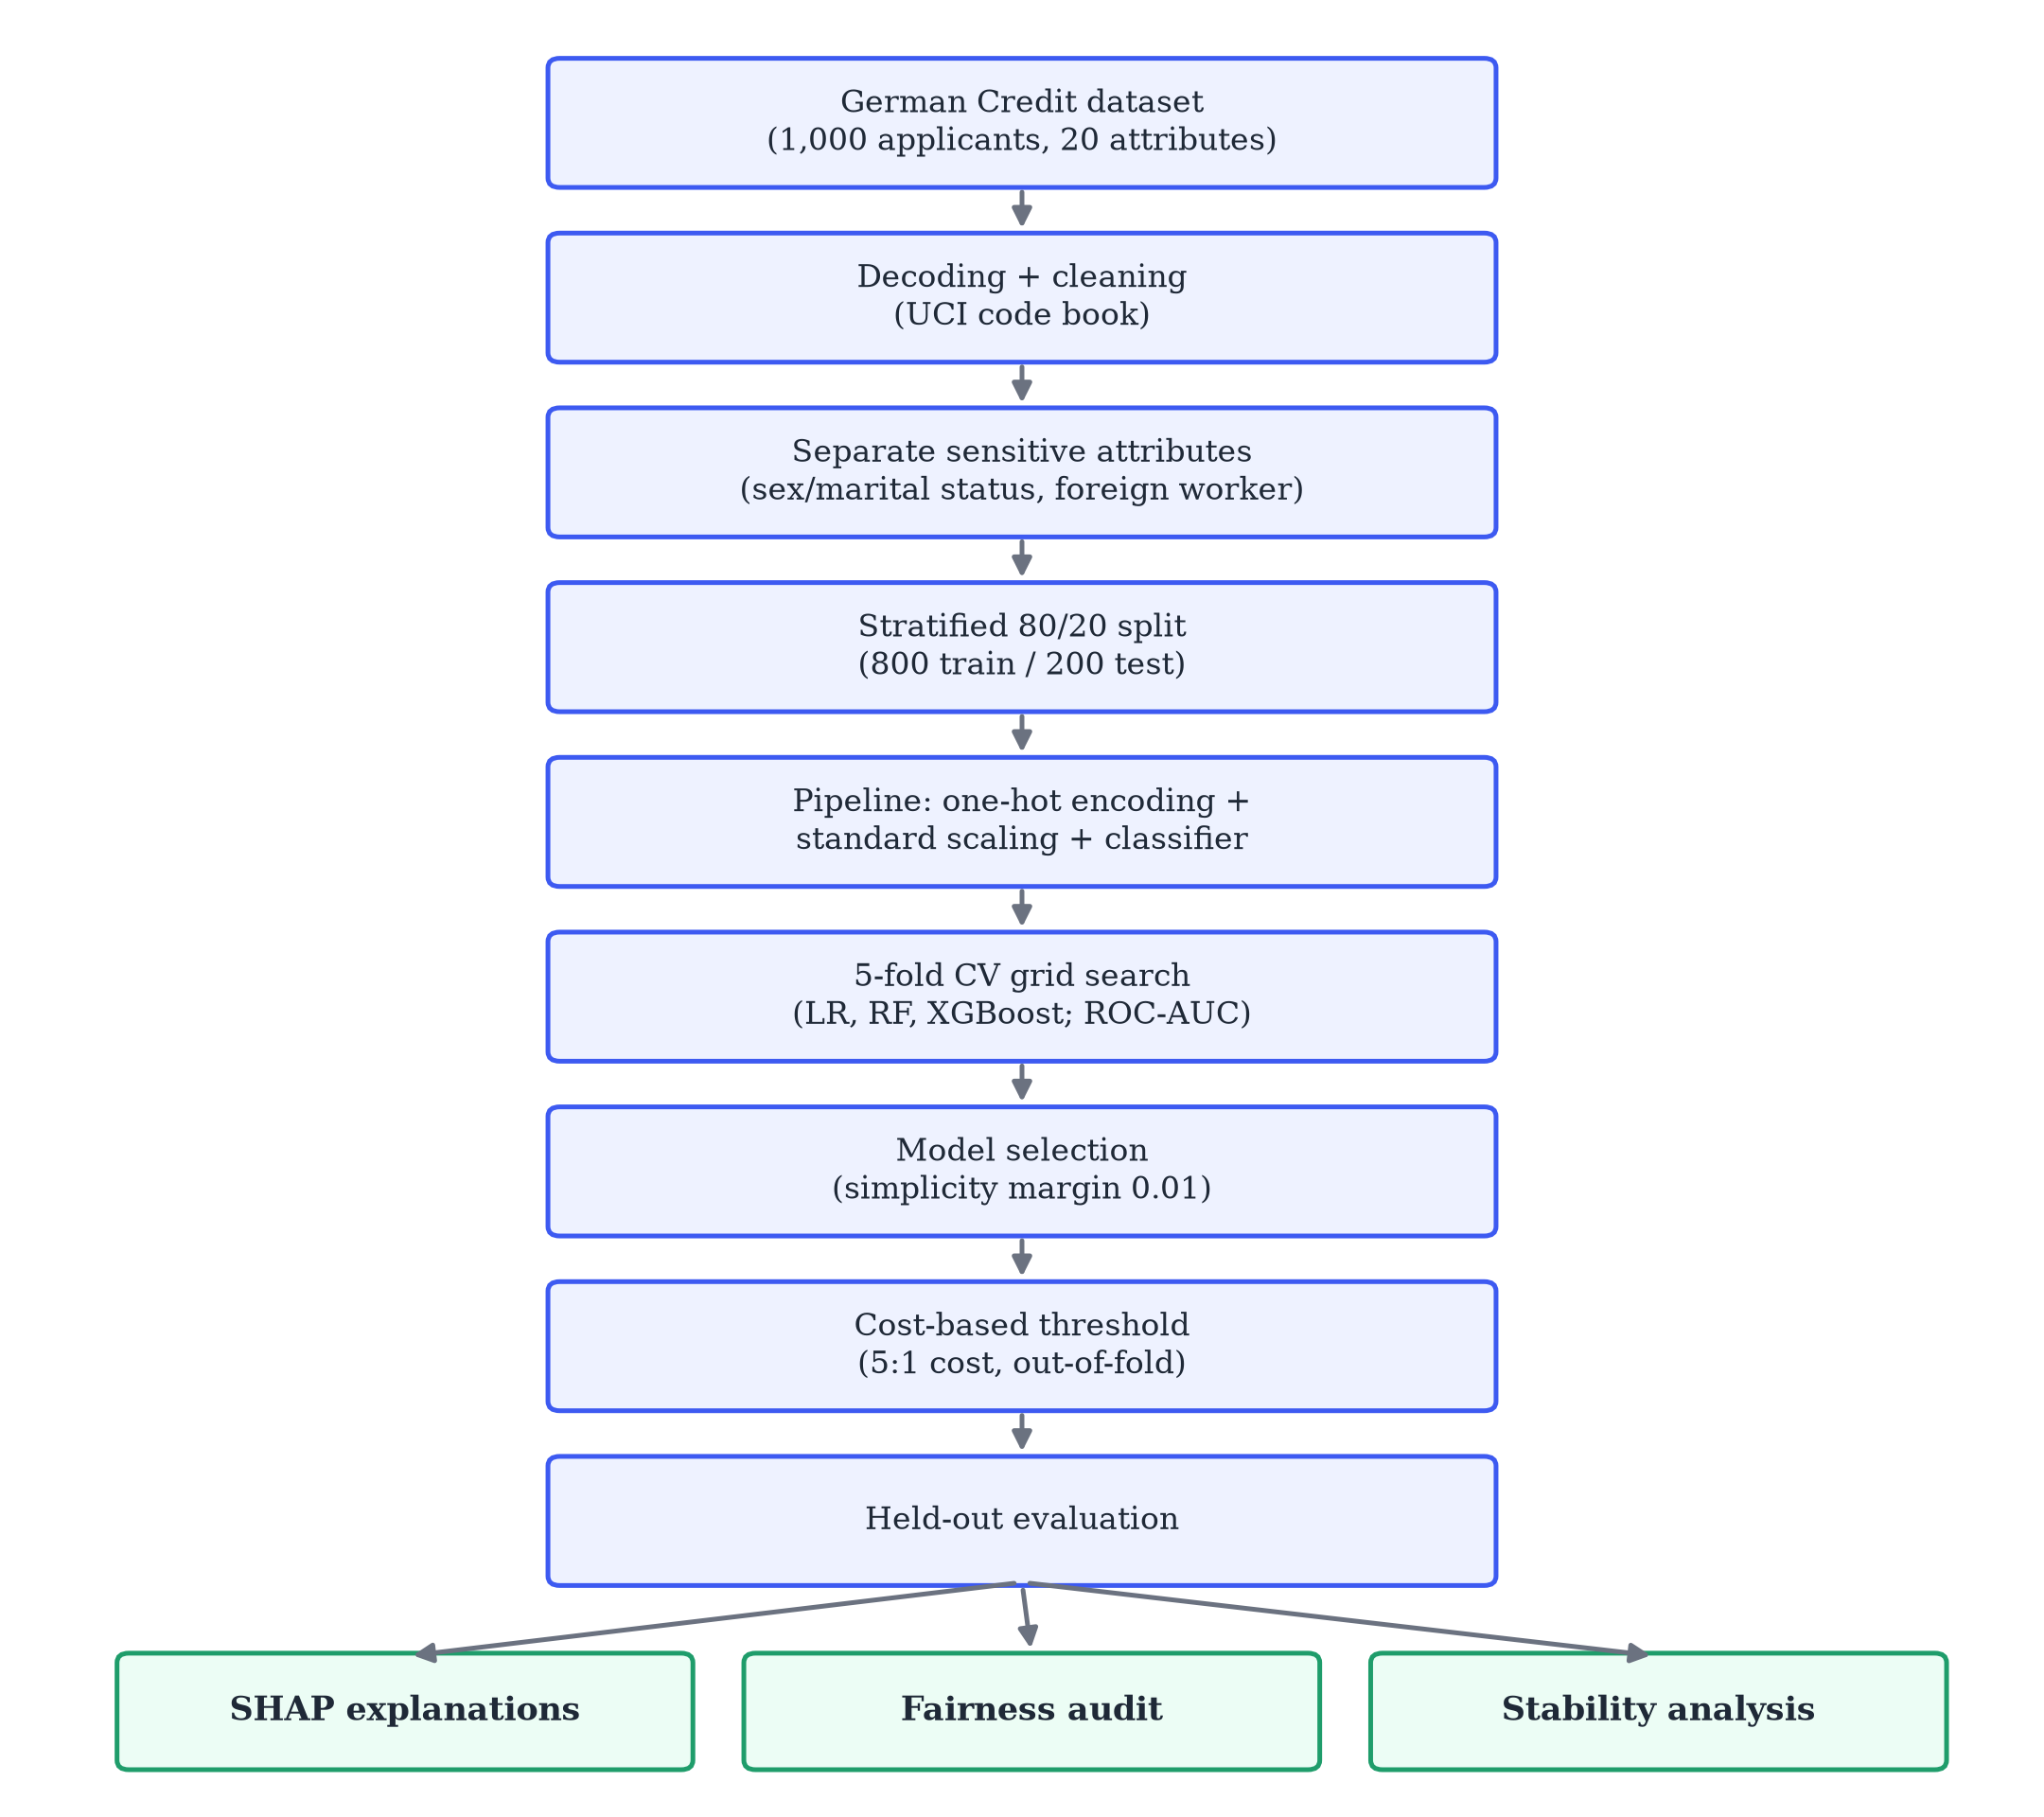
\includegraphics[width=0.8\textwidth,height=\textheight]{figures/methodology.png}
\caption{Methodology pipeline of the proposed framework.}
\end{figure}

\hypertarget{dataset-description}{%
\section{8. Dataset Description}\label{dataset-description}}

The Statlog German Credit dataset {[}14{]} contains 1,000 loan
applicants described by 20 attributes and a binary target: 700
applicants are labelled good credit risks and 300 bad. Seven attributes
are numeric (loan duration in months, credit amount, installment rate as
a percentage of disposable income, years at current residence, age,
number of existing credits at the bank and number of dependants) and
thirteen are categorical (checking-account status, credit history, loan
purpose, savings, employment duration, personal status and sex, other
debtors or guarantors, property, other installment plans, housing, job,
telephone and foreign-worker status). Monetary values are in Deutsche
Mark (DM). There are no missing values.

The raw file encodes categorical values as symbolic codes (for example
\texttt{A11} for a checking-account balance below 0 DM). We decode these
using the code book distributed with the dataset so that model inputs,
explanations and the user interface use readable values.

\textbf{Sensitive attributes.} The dataset contains three attributes
commonly treated as sensitive: \emph{personal status and sex},
\emph{age} and \emph{foreign worker}. The personal-status attribute
mixes marital status and sex, and the code for ``female, single'' does
not occur in the data; we therefore derive a binary \texttt{sex}
variable (female / male) for auditing only. Only 37 of the 1,000
applicants are not foreign workers. The dataset documentation also
supplies a cost matrix in which classifying a bad applicant as good
costs 5 and classifying a good applicant as bad costs 1 {[}14{]}.

\hypertarget{data-preprocessing}{%
\section{9. Data Preprocessing}\label{data-preprocessing}}

\begin{enumerate}
\def\labelenumi{\arabic{enumi}.}
\tightlist
\item
  \textbf{Decoding and validation.} Every symbolic code is mapped to its
  documented meaning; an unknown code raises an error rather than being
  silently accepted.
\item
  \textbf{Target.} The original label (1 = good, 2 = bad) is converted
  to \texttt{is\_bad} \(\in \{0, 1\}\), so the positive class is the
  high-risk outcome.
\item
  \textbf{Cleaning.} Duplicates are removed (none were found) and
  numeric columns are type-checked. Median and mode imputation are
  included for robustness, although the dataset has no missing values.
\item
  \textbf{Sensitive-attribute handling.} \texttt{personal\_status\_sex}
  and \texttt{foreign\_worker} are excluded from the model inputs and
  retained only for the fairness audit. Age is kept as a model feature,
  because it is widely used in credit scoring, but it is audited
  explicitly. The model therefore uses 18 features: 7 numeric and 11
  categorical.
\item
  \textbf{Encoding and scaling.} Categorical features are one-hot
  encoded (unknown categories are ignored at prediction time) and
  numeric features are standardised, giving 55 model columns. Scaling is
  necessary for logistic regression and harmless for tree models, so one
  preprocessing definition is shared by all candidates.
\item
  \textbf{Split.} A stratified 80/20 split with a fixed random seed
  yields 800 training and 200 test applicants, preserving the 70/30
  class ratio.
\end{enumerate}

\hypertarget{machine-learning-models}{%
\section{10. Machine Learning Models}\label{machine-learning-models}}

\textbf{Logistic regression (LR)} models the log-odds of default as a
linear function of the encoded features \(\mathbf{x}\):

\[P(y=1 \mid \mathbf{x}) = \sigma(\mathbf{w}^\top \mathbf{x} + b) = \frac{1}{1 + e^{-(\mathbf{w}^\top \mathbf{x} + b)}}\]

with L2 regularisation strength controlled by \(C\). It serves as the
transparent baseline traditionally used in scorecards.

\textbf{Random forest (RF)} {[}12{]} averages the class-probability
estimates of \(T\) decision trees, each grown on a bootstrap sample of
the training data with a random subset of features considered at each
split:

\[\hat{p}(\mathbf{x}) = \frac{1}{T} \sum_{t=1}^{T} p_t(\mathbf{x})\]

Averaging many decorrelated trees reduces variance compared with a
single tree.

\textbf{XGBoost} {[}13{]} builds trees sequentially, each fitted to the
gradient of the loss of the current ensemble, with shrinkage (learning
rate) and regularisation to control overfitting.

Hyper-parameter grids were kept small to suit the dataset size:
\(C \in \{0.01, 0.1, 0.3, 1, 3\}\) for LR; 300 trees with maximum depth
\(\in \{4, 8, \text{none}\}\) and minimum leaf size \(\in \{1, 5\}\) for
RF; and for XGBoost, 100 or 300 trees, maximum depth
\(\in \{2, 3, 4\}\), learning rate \(\in \{0.03, 0.1\}\) and subsample
0.8.

\hypertarget{model-selection-and-evaluation-metrics}{%
\section{11. Model Selection and Evaluation
Metrics}\label{model-selection-and-evaluation-metrics}}

\hypertarget{metrics}{%
\subsection{11.1 Metrics}\label{metrics}}

With \(TP\), \(FP\), \(TN\) and \(FN\) denoting true/false
positives/negatives (positive = bad credit):

\[\text{Precision} = \frac{TP}{TP+FP}, \quad \text{Recall} = \frac{TP}{TP+FN}, \quad F_1 = \frac{2\,\text{Precision}\cdot\text{Recall}}{\text{Precision}+\text{Recall}}\]

ROC-AUC is the area under the curve of true-positive rate against
false-positive rate as the threshold varies; it equals the probability
that a randomly chosen bad applicant receives a higher risk score than a
randomly chosen good applicant {[}26{]}. We also report the dataset's
misclassification cost, \(\text{Cost} = 5\,FN + 1\,FP\).

Accuracy alone is unsuitable here. Because 70\% of applicants are good,
a model that approves everyone reaches 70\% accuracy while identifying
no defaulters. Recall measures how many defaulters are caught; precision
measures how many flagged applicants are truly risky; ROC-AUC measures
ranking quality independently of any threshold.

\hypertarget{selection-rule}{%
\subsection{11.2 Selection rule}\label{selection-rule}}

Models were compared on mean five-fold cross-validated ROC-AUC computed
on the training set only. The model with the highest score is selected
unless a simpler model lies within 0.01 of it, in which case the simpler
model is preferred (order of simplicity: LR, RF, XGBoost). This margin
reflects the fact that differences smaller than about 0.01 AUC are well
within the fold-to-fold variation for 800 training examples.

\hypertarget{cost-based-decision-threshold}{%
\subsection{11.3 Cost-based decision
threshold}\label{cost-based-decision-threshold}}

A default threshold of 0.5 implicitly treats both errors as equally
costly. Under the 5:1 cost matrix, decision theory suggests flagging an
applicant when the expected cost of approval exceeds that of rejection,
i.e.~when \(5p > 1(1-p)\), or \(p > 1/6\), assuming perfectly calibrated
probabilities {[}27{]}. Random-forest probabilities are not perfectly
calibrated, so instead of using this theoretical value we search
thresholds from 0.05 to 0.95 in steps of 0.01 and choose the one that
minimises \(5\,FN + FP\) on \emph{out-of-fold} predictions for the
training set (obtained with \texttt{cross\_val\_predict}). The test set
plays no part in this choice.

For presentation, predicted probabilities are additionally grouped into
three bands: \textbf{LOW} (\(p <\) threshold), \textbf{MEDIUM}
(threshold \(\le p < 0.5\); flagged but borderline, recommended for
human review) and \textbf{HIGH} (\(p \ge 0.5\)).

\hypertarget{explainable-ai-using-shap}{%
\section{12. Explainable AI Using
SHAP}\label{explainable-ai-using-shap}}

SHAP {[}6{]} explains a prediction \(f(\mathbf{x})\) as a sum of feature
contributions added to a base value:

\[f(\mathbf{x}) = \phi_0 + \sum_{j=1}^{M} \phi_j\]

where \(\phi_0\) is the expected model output over a background dataset
and \(\phi_j\) is the Shapley value of feature \(j\), i.e.~its average
marginal contribution over all subsets of the other features. We use the
TreeSHAP algorithm {[}18{]} in interventional mode with 100 randomly
selected training applicants as background, and explain the model's
output in probability units.

Because the model operates on one-hot encoded columns while users think
in terms of original attributes, the SHAP values of all columns derived
from the same attribute are summed. This is valid because Shapley values
are additive. A positive value means the attribute pushed the estimated
default probability \textbf{up} (towards high risk); a negative value
means it pushed the probability \textbf{down}. Global importance is the
mean absolute SHAP value of each attribute over the 200 test applicants.
An automated test checks that \(\phi_0 + \sum_j \phi_j\) reproduces the
predicted probability to within 0.01.

\hypertarget{fairness-analysis}{%
\section{13. Fairness Analysis}\label{fairness-analysis}}

For each sensitive grouping \(A\) --- derived sex, age group (under 25 /
25 and over) and foreign-worker status --- the audit computes, on the
test set and at the deployed threshold, per-group counts, approval rates
(share predicted low risk), false-positive rates (good payers wrongly
flagged), false-negative rates (bad payers approved), accuracy and the
observed good-credit rate. Using Fairlearn's \texttt{MetricFrame}
{[}23{]}, two summary measures are reported:

\[\text{DPD} = \max_{a} P(\hat{Y}=1 \mid A=a) - \min_{a} P(\hat{Y}=1 \mid A=a)\]

\[\text{EOD} = \max\Big(\max_{a,b}\big|TPR_a - TPR_b\big|,\ \max_{a,b}\big|FPR_a - FPR_b\big|\Big)\]

DPD (demographic parity difference) measures the largest gap in
selection rates between groups and EOD (equalized odds difference)
{[}20{]} measures the largest gap in either error rate. The demographic
parity ratio (smallest over largest selection rate) is also reported. As
a reporting heuristic, a grouping is labelled ACCEPTABLE if
\(\max(\text{DPD}, \text{EOD}) < 0.10\), NEEDS ATTENTION if it is below
0.20, and CONCERNING otherwise; groups with fewer than 30 test
applicants are flagged as unreliable. These labels are descriptive aids,
not legal standards, and passing them would not establish that the model
is fair {[}21{]}, {[}22{]}. No re-weighting, resampling or
post-processing was applied.

\hypertarget{prediction-stability-and-robustness}{%
\section{14. Prediction Stability and
Robustness}\label{prediction-stability-and-robustness}}

The stability test asks whether a decision survives small, plausible
variations in the applicant's numbers. For an applicant \(\mathbf{x}\)
with decision \(d(\mathbf{x})\):

\begin{enumerate}
\def\labelenumi{\arabic{enumi}.}
\tightlist
\item
  \textbf{Random perturbation.} Generate \(N = 20\) copies in which loan
  duration and credit amount are multiplied by \((1+\varepsilon)\) with
  \(\varepsilon \sim \mathcal{N}(0, 0.05^2)\), rounded and clipped to
  valid ranges. Stability is the fraction of copies receiving the same
  decision:
  \[S(\mathbf{x}) = \frac{1}{N}\sum_{i=1}^{N} \mathbb{1}\big[d(\tilde{\mathbf{x}}_i) = d(\mathbf{x})\big]\]
\item
  \textbf{One-at-a-time sensitivity.} Change each non-sensitive numeric
  feature individually (±5\% and ±10\% for duration and amount; ±1 step
  for the small integer scales of installment rate, residence, existing
  credits and dependants) and record the largest change in predicted
  probability and whether the decision flips.
\end{enumerate}

Age is deliberately not perturbed: asking how a decision changes with
age is a fairness question rather than a robustness question. This is a
basic local robustness check, not a certification of adversarial
robustness {[}24{]}. A fixed random seed makes results reproducible.

\hypertarget{system-architecture}{%
\section{15. System Architecture}\label{system-architecture}}

The system follows a simple client-server design (Fig. 2). A React
single-page application calls a FastAPI backend over REST. The backend
validates every request with Pydantic schemas generated from the dataset
code book, so out-of-range numbers and unknown categories are rejected
with field-level error messages. Four service modules implement
prediction, SHAP explanation, the fairness audit and the stability test.
Training is a separate offline script whose artefacts (the fitted
pipeline, metadata, feature schema, SHAP background sample and test set)
are loaded once when the API starts. Assessment records are kept in an
in-memory store containing only the decision, the top contributing
factors and a hash of the input; raw applicant data are not retained.

\begin{figure}
\centering
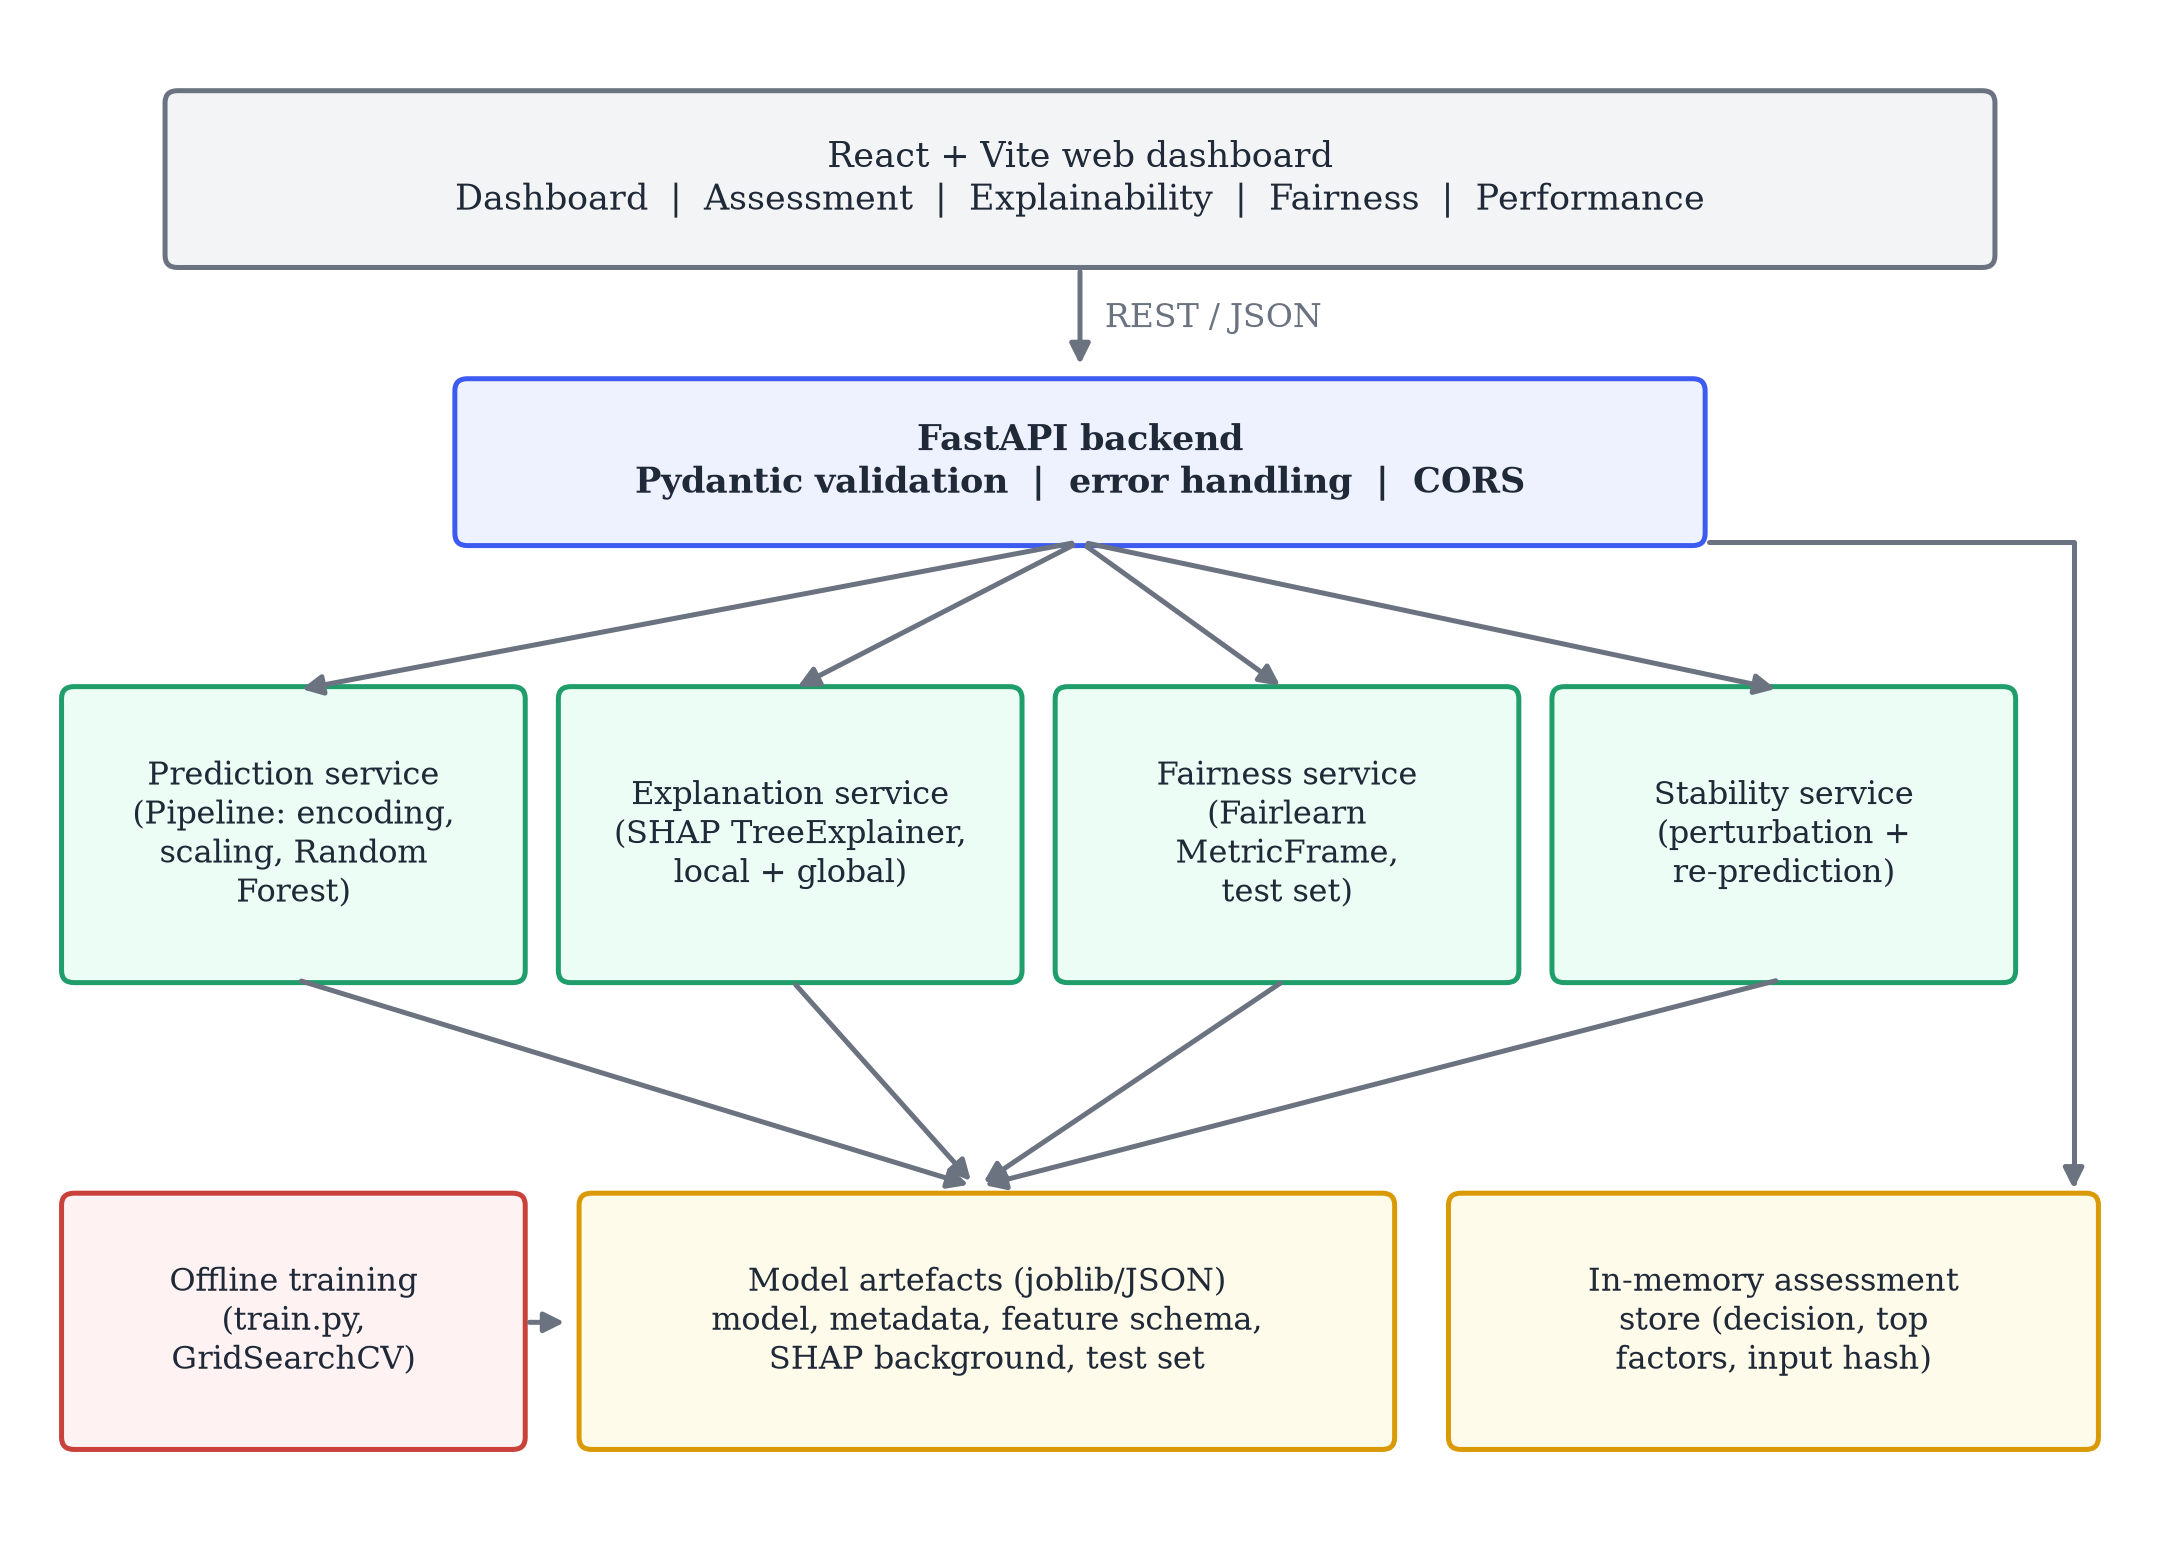
\includegraphics[width=0.95\textwidth,height=\textheight]{figures/system_architecture.png}
\caption{System architecture of the prototype.}
\end{figure}

\hypertarget{implementation}{%
\section{16. Implementation}\label{implementation}}

The ML components use Python with pandas, NumPy, scikit-learn {[}25{]},
XGBoost {[}13{]}, SHAP {[}6{]} and Fairlearn {[}23{]}. The REST API
exposes endpoints for health checks, prediction, full explanation,
stability analysis, the fairness report, model metrics, the input
schema, global importance and assessment history; interactive OpenAPI
documentation is generated automatically.

The web dashboard has five views:

\begin{itemize}
\tightlist
\item
  \textbf{Dashboard:} session statistics, model metrics and a fairness
  summary.
\item
  \textbf{Credit Assessment:} an input form generated from the model's
  own feature schema, so the interface cannot ask for attributes the
  model does not use. Results include the decision, a probability bar
  marked with the threshold, plain-language lists of risk-increasing and
  risk-reducing factors, a SHAP chart, the stability test and a
  printable report.
\item
  \textbf{Explainability:} local and global SHAP charts.
\item
  \textbf{Fairness:} per-group charts and tables with interpretations
  and limitations.
\item
  \textbf{Model Performance:} confusion matrix and model comparison.
\end{itemize}

Docker Compose files are provided for containerised execution, and a
Jupyter notebook reproduces the exploratory analysis. The code base
includes 19 automated backend tests (preprocessing, SHAP additivity, API
behaviour, input validation and privacy of stored records) and 8
frontend component tests. All random seeds are fixed at 42.

\hypertarget{experimental-results}{%
\section{17. Experimental Results}\label{experimental-results}}

\hypertarget{model-comparison}{%
\subsection{17.1 Model comparison}\label{model-comparison}}

Table I reports cross-validated ROC-AUC on the training set and test-set
metrics for each tuned model at the default 0.5 threshold. All values
are taken from the saved training output.

\textbf{Table I. Model comparison (CV on 800 training applicants; test
metrics on 200 applicants at threshold 0.5)}

\begin{longtable}[]{@{}
  >{\raggedright\arraybackslash}p{(\columnwidth - 14\tabcolsep) * \real{0.2911}}
  >{\raggedleft\arraybackslash}p{(\columnwidth - 14\tabcolsep) * \real{0.1013}}
  >{\raggedleft\arraybackslash}p{(\columnwidth - 14\tabcolsep) * \real{0.1013}}
  >{\raggedleft\arraybackslash}p{(\columnwidth - 14\tabcolsep) * \real{0.1013}}
  >{\raggedleft\arraybackslash}p{(\columnwidth - 14\tabcolsep) * \real{0.1013}}
  >{\raggedleft\arraybackslash}p{(\columnwidth - 14\tabcolsep) * \real{0.1013}}
  >{\raggedleft\arraybackslash}p{(\columnwidth - 14\tabcolsep) * \real{0.1013}}
  >{\raggedleft\arraybackslash}p{(\columnwidth - 14\tabcolsep) * \real{0.1013}}@{}}
\toprule\noalign{}
\begin{minipage}[b]{\linewidth}\raggedright
Model
\end{minipage} & \begin{minipage}[b]{\linewidth}\raggedleft
CV ROC-AUC
\end{minipage} & \begin{minipage}[b]{\linewidth}\raggedleft
Accuracy
\end{minipage} & \begin{minipage}[b]{\linewidth}\raggedleft
Precision
\end{minipage} & \begin{minipage}[b]{\linewidth}\raggedleft
Recall
\end{minipage} & \begin{minipage}[b]{\linewidth}\raggedleft
F1
\end{minipage} & \begin{minipage}[b]{\linewidth}\raggedleft
Test ROC-AUC
\end{minipage} & \begin{minipage}[b]{\linewidth}\raggedleft
Cost
\end{minipage} \\
\midrule\noalign{}
\endhead
\bottomrule\noalign{}
\endlastfoot
Logistic Regression & 0.7749 & 0.770 & 0.694 & 0.417 & 0.521 & 0.809 &
186 \\
Random Forest & 0.7923 & 0.765 & 0.724 & 0.350 & 0.472 & 0.809 & 203 \\
XGBoost & 0.7965 & 0.775 & 0.683 & 0.467 & 0.555 & 0.806 & 173 \\
\end{longtable}

Selected hyper-parameters: LR \(C\) = 0.1; RF 300 trees, maximum depth
8, minimum leaf size 5; XGBoost 300 trees, maximum depth 4, learning
rate 0.03, subsample 0.8.

\begin{figure}
\centering
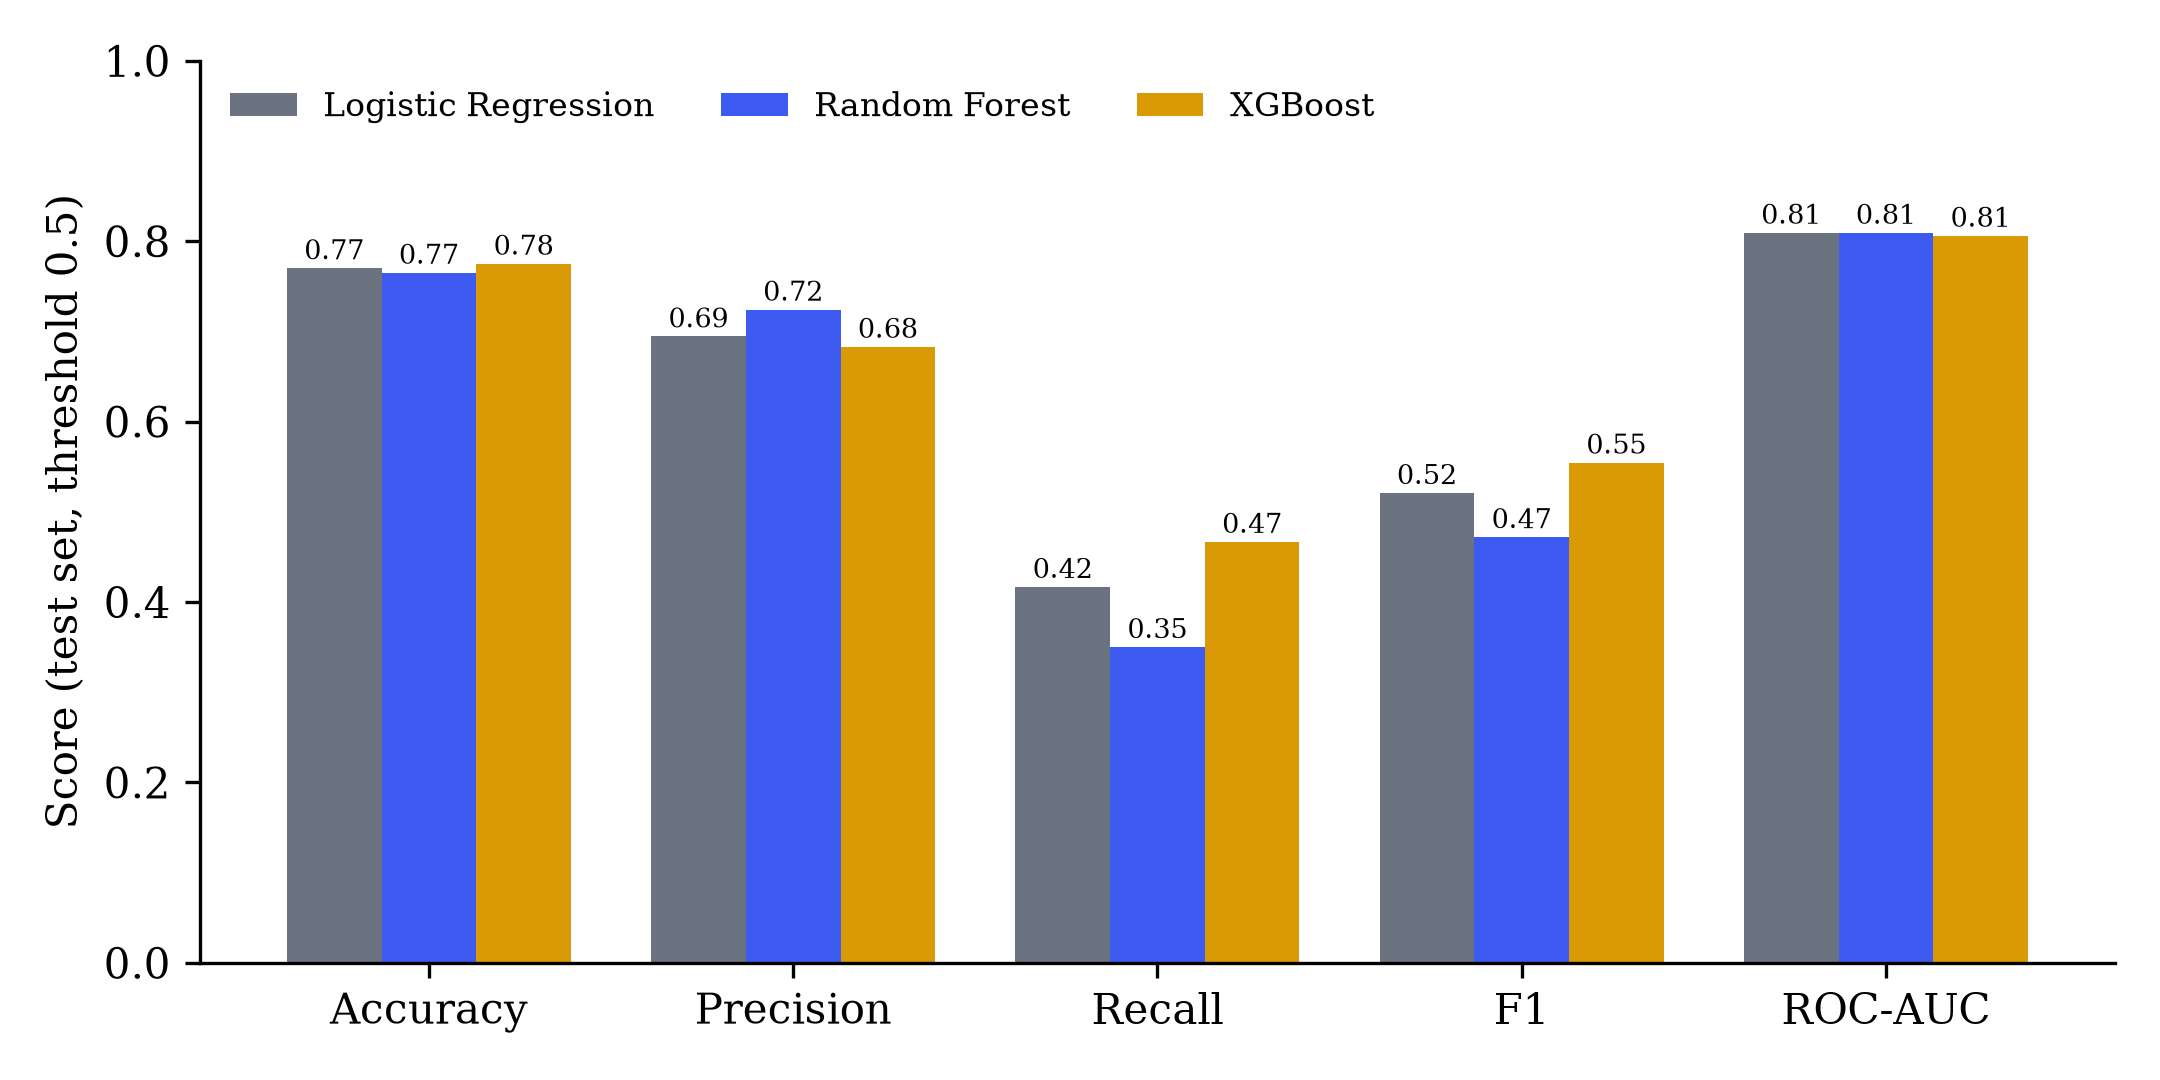
\includegraphics[width=0.9\textwidth,height=\textheight]{figures/model_comparison.png}
\caption{Test-set metrics of the three candidate models at
threshold 0.5.}
\end{figure}

The three models are close: test ROC-AUC ranges only from 0.806 to
0.809, and cross-validated ROC-AUC from 0.775 to 0.797. XGBoost achieved
the highest cross-validated score, but the random forest was within
0.0042 and was therefore selected under the simplicity rule of Section
11.2. Given the small differences, we do not claim that any of the three
models is clearly superior on this dataset.

At the default threshold of 0.5, all models miss most defaulters (recall
between 0.35 and 0.47). This illustrates why the threshold matters as
much as the choice of model for this task.

\hypertarget{selected-model-at-the-cost-based-threshold}{%
\subsection{17.2 Selected model at the cost-based
threshold}\label{selected-model-at-the-cost-based-threshold}}

The out-of-fold search selected a threshold of \textbf{0.27}. Table II
shows the random forest's held-out performance at this threshold.

\textbf{Table II. Random forest on the held-out test set at threshold
0.27}

\begin{longtable}[]{@{}rrrrrr@{}}
\toprule\noalign{}
Accuracy & Precision & Recall & F1 & ROC-AUC & Cost (5·FN + FP) \\
\midrule\noalign{}
\endhead
\bottomrule\noalign{}
\endlastfoot
0.640 & 0.447 & 0.850 & 0.586 & 0.809 & 108 \\
\end{longtable}

\textbf{Table III. Confusion matrix (positive = bad credit)}

\begin{longtable}[]{@{}lrr@{}}
\toprule\noalign{}
& Predicted low risk & Predicted high risk \\
\midrule\noalign{}
\endhead
\bottomrule\noalign{}
\endlastfoot
\textbf{Actually good (140)} & 77 (TN) & 63 (FP) \\
\textbf{Actually bad (60)} & 9 (FN) & 51 (TP) \\
\end{longtable}

Lowering the threshold from 0.5 to 0.27 raised recall from 0.350 to
0.850 (51 of 60 defaulters identified) and reduced the cost from 203 to
108. The price is a lower precision (0.447) and accuracy (0.640): 63 of
140 good applicants are flagged. This is the trade-off implied by the
5:1 cost matrix, and it is why accuracy should not be read in isolation.
Because these figures come from a single 200-applicant test set, they
carry considerable sampling uncertainty; confidence intervals are left
for future work.

\hypertarget{explainability-results}{%
\subsection{17.3 Explainability results}\label{explainability-results}}

\textbf{Global importance.} Fig. 4 shows the mean absolute SHAP values
over the test set. The five most influential attributes are
checking-account status (0.086), loan duration (0.032), savings (0.027),
credit history (0.023) and credit amount (0.019). Age ranks eleventh
(0.011). Dependants, existing credits and years at residence contribute
least.

\begin{figure}
\centering
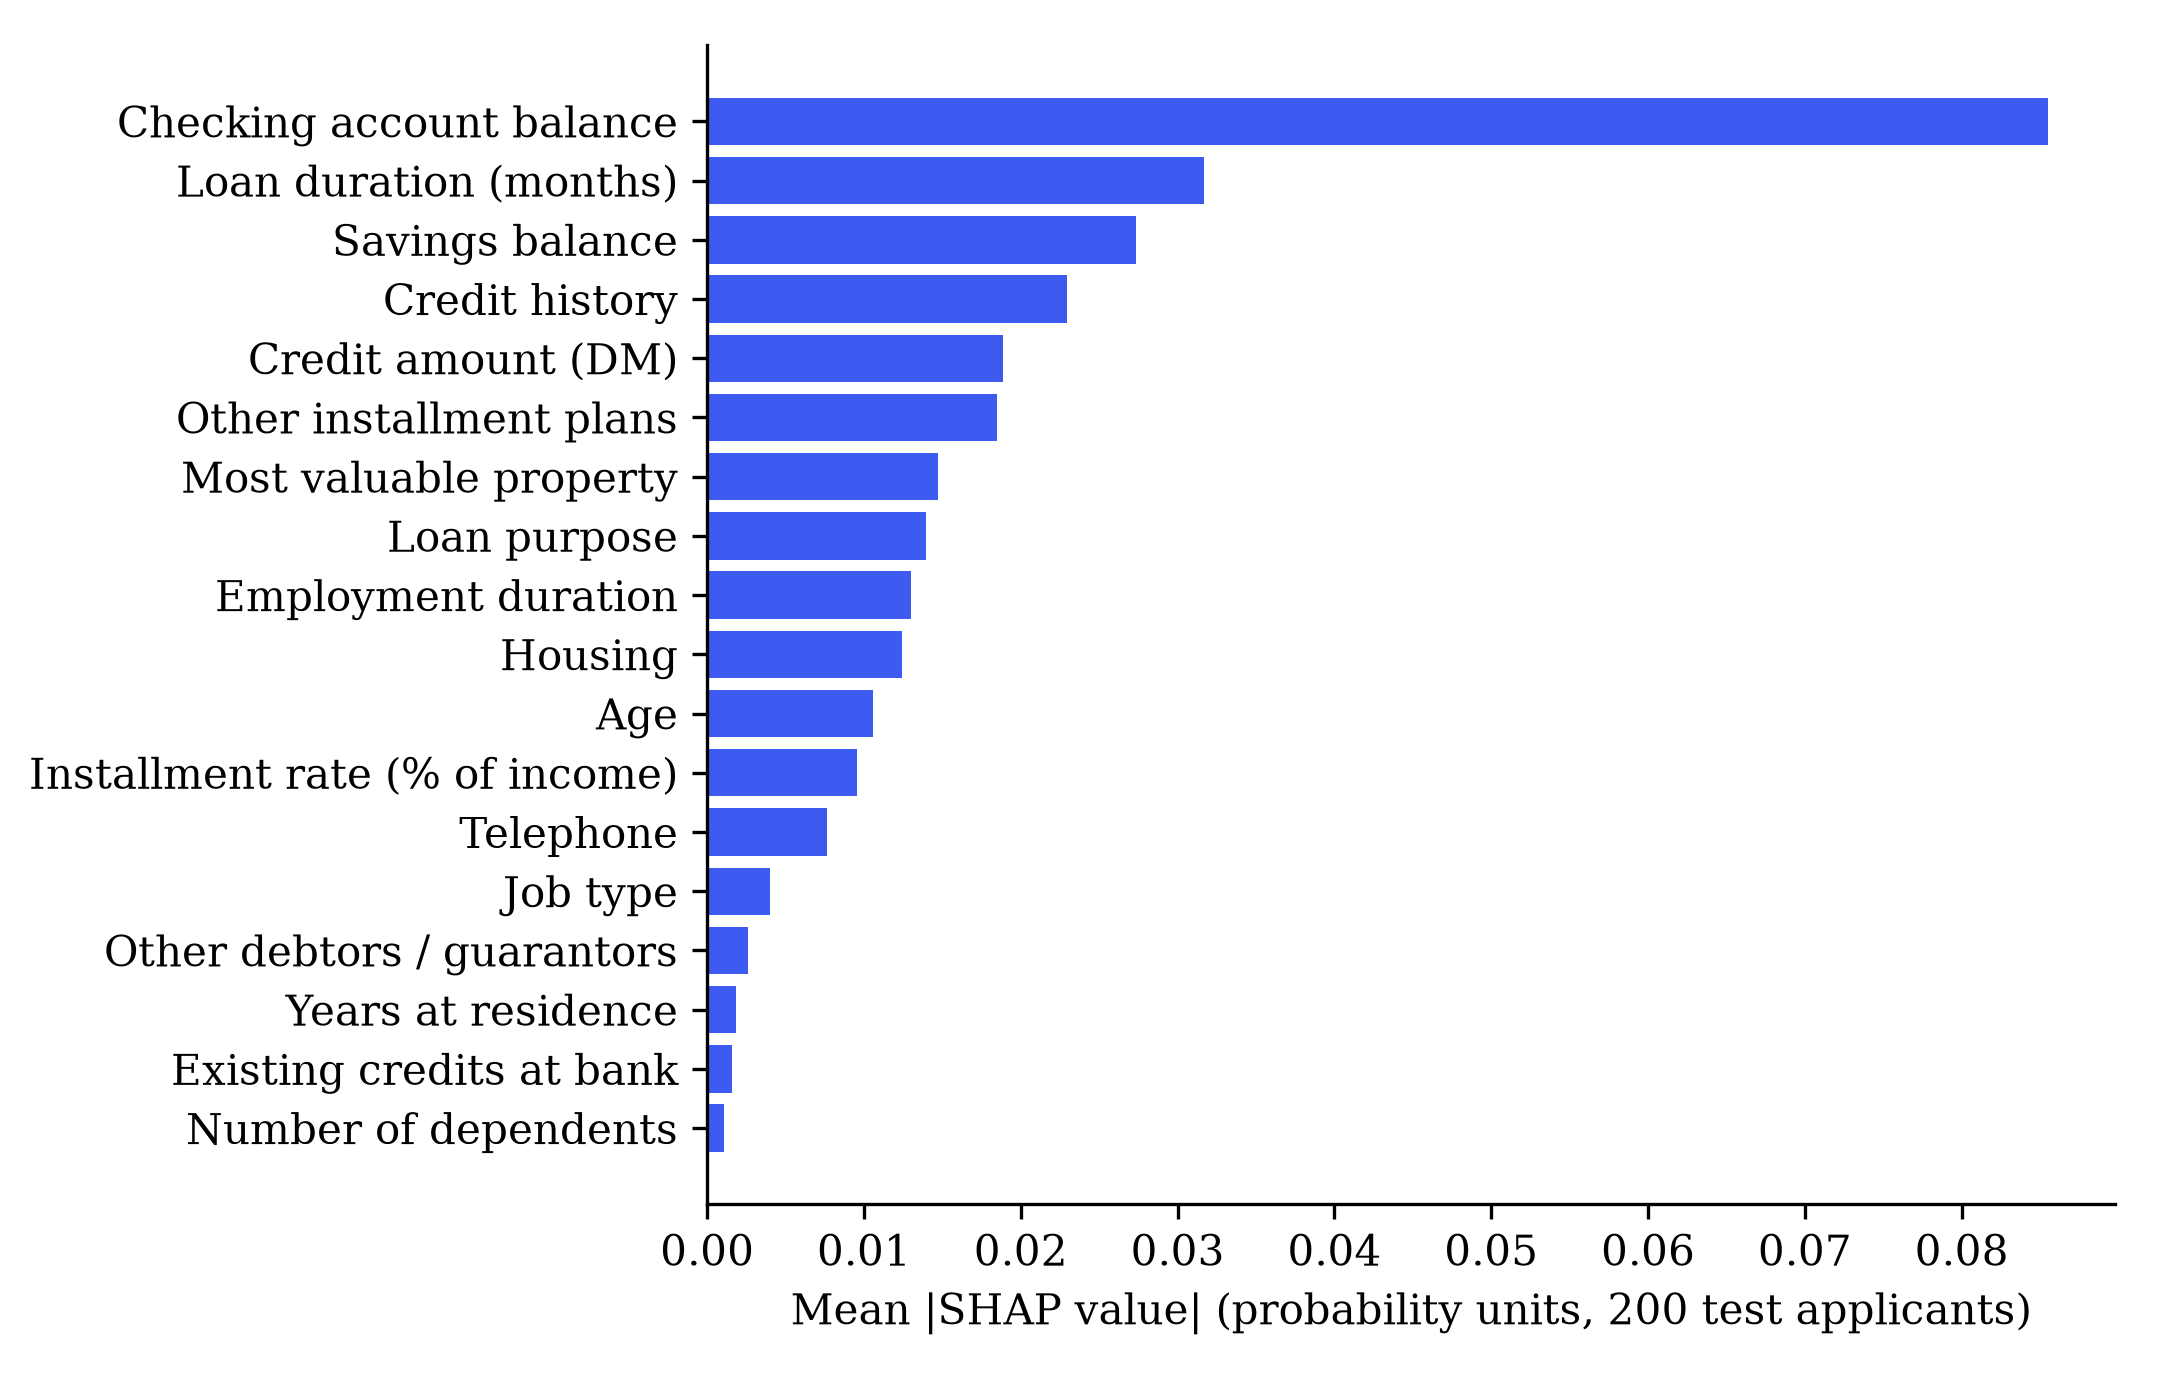
\includegraphics[width=0.9\textwidth,height=\textheight]{figures/shap_global_importance.png}
\caption{Global feature importance (mean absolute SHAP value,
probability units, 200 test applicants).}
\end{figure}

\textbf{Local explanation example.} Table IV shows the actual
explanation produced by the system for a borderline applicant: a
24-month furniture loan of 2,500 DM, checking balance 0--200 DM, savings
below 100 DM, installment rate 4, age 30, skilled employee and home
owner. The base value \(\phi_0\) (mean predicted probability over the
background sample) is 0.299, and the model predicts 0.412. This is above
the 0.27 threshold but below 0.5, so the decision is HIGH RISK in the
MEDIUM band, a case the interface recommends for human review.

\textbf{Table IV. Largest SHAP contributions for the borderline
applicant (actual system output)}

\begin{longtable}[]{@{}
  >{\raggedright\arraybackslash}p{(\columnwidth - 6\tabcolsep) * \real{0.2308}}
  >{\raggedright\arraybackslash}p{(\columnwidth - 6\tabcolsep) * \real{0.2308}}
  >{\raggedleft\arraybackslash}p{(\columnwidth - 6\tabcolsep) * \real{0.3077}}
  >{\raggedright\arraybackslash}p{(\columnwidth - 6\tabcolsep) * \real{0.2308}}@{}}
\toprule\noalign{}
\begin{minipage}[b]{\linewidth}\raggedright
Attribute
\end{minipage} & \begin{minipage}[b]{\linewidth}\raggedright
Value
\end{minipage} & \begin{minipage}[b]{\linewidth}\raggedleft
SHAP
\end{minipage} & \begin{minipage}[b]{\linewidth}\raggedright
Effect
\end{minipage} \\
\midrule\noalign{}
\endhead
\bottomrule\noalign{}
\endlastfoot
Checking account balance & 0--200 DM & +0.050 & increases risk \\
Savings balance & \textless{} 100 DM & +0.038 & increases risk \\
Loan duration & 24 months & +0.023 & increases risk \\
Credit amount & 2,500 DM & −0.021 & reduces risk \\
Credit history & existing credits paid duly & +0.011 & increases risk \\
Installment rate & 4 (highest) & +0.010 & increases risk \\
Housing & own & −0.010 & reduces risk \\
Other installment plans & none & −0.009 & reduces risk \\
\end{longtable}

The remaining ten attributes each contribute less than 0.01 in absolute
value. The explanation is easy to read: a modest checking balance, very
low savings and the highest installment burden push the risk up, while a
relatively small loan and home ownership pull it down. The two other
sample applicants built into the demo give the expected contrast: a
``typical good'' profile receives 0.104 (LOW), and a ``risky'' profile
(overdrawn account, 60-month 15,000 DM loan, under one year of
employment) receives 0.748 (HIGH).

\hypertarget{stability-results}{%
\subsection{17.4 Stability results}\label{stability-results}}

The stability test was run for all 200 test applicants with \(N = 20\)
perturbations, noise level 5\% and seed 42 (script provided in the
paper's \texttt{scripts} folder).

\textbf{Table V. Stability of decisions on the test set}

\begin{longtable}[]{@{}
  >{\raggedright\arraybackslash}p{(\columnwidth - 2\tabcolsep) * \real{0.4286}}
  >{\raggedleft\arraybackslash}p{(\columnwidth - 2\tabcolsep) * \real{0.5714}}@{}}
\toprule\noalign{}
\begin{minipage}[b]{\linewidth}\raggedright
Measure
\end{minipage} & \begin{minipage}[b]{\linewidth}\raggedleft
Result
\end{minipage} \\
\midrule\noalign{}
\endhead
\bottomrule\noalign{}
\endlastfoot
Mean stability score \(\bar{S}\) & 0.995 \\
Applicants with \(S = 1\) (all 20 copies unchanged) & 193 / 200
(96.5\%) \\
Applicants with \(S \ge 0.9\) & 198 / 200 (99.0\%) \\
Lowest individual stability score & 0.55 \\
Applicants for whom a one-feature change flips the decision & 9 / 200
(4.5\%) \\
Mean stability, applicants within ±0.05 of the threshold (n = 38) &
0.974 \\
Mean stability, all other applicants (n = 162) & 1.000 \\
\end{longtable}

Decisions were highly stable overall, and every instability occurred for
applicants whose probability lay close to the threshold. Among the
single-feature changes that flipped a decision, loan duration was
involved most often (6 flips), followed by number of dependants (3),
credit amount (2) and installment rate (2). In other words, instability
is concentrated in genuinely borderline cases, which supports routing
such cases to human review rather than relying on the automated
decision. The three demo applicants all had a stability score of 1.0.

\hypertarget{fairness-results}{%
\section{18. Fairness Results}\label{fairness-results}}

\textbf{Table VI. Group metrics on the test set at threshold 0.27
(Fairlearn)}

\begin{longtable}[]{@{}
  >{\raggedright\arraybackslash}p{(\columnwidth - 10\tabcolsep) * \real{0.1364}}
  >{\raggedright\arraybackslash}p{(\columnwidth - 10\tabcolsep) * \real{0.1364}}
  >{\raggedleft\arraybackslash}p{(\columnwidth - 10\tabcolsep) * \real{0.1818}}
  >{\raggedleft\arraybackslash}p{(\columnwidth - 10\tabcolsep) * \real{0.1818}}
  >{\raggedleft\arraybackslash}p{(\columnwidth - 10\tabcolsep) * \real{0.1818}}
  >{\raggedleft\arraybackslash}p{(\columnwidth - 10\tabcolsep) * \real{0.1818}}@{}}
\toprule\noalign{}
\begin{minipage}[b]{\linewidth}\raggedright
Attribute
\end{minipage} & \begin{minipage}[b]{\linewidth}\raggedright
Group (n)
\end{minipage} & \begin{minipage}[b]{\linewidth}\raggedleft
Approval rate
\end{minipage} & \begin{minipage}[b]{\linewidth}\raggedleft
Actual good rate
\end{minipage} & \begin{minipage}[b]{\linewidth}\raggedleft
FPR (good payers rejected)
\end{minipage} & \begin{minipage}[b]{\linewidth}\raggedleft
FNR (bad payers approved)
\end{minipage} \\
\midrule\noalign{}
\endhead
\bottomrule\noalign{}
\endlastfoot
Sex & female (61) & 41.0\% & 67.2\% & 51.2\% & 25.0\% \\
& male (139) & 43.9\% & 71.2\% & 42.4\% & 10.0\% \\
Age & 25 and over (161) & 47.8\% & 74.5\% & 40.8\% & 14.6\% \\
& under 25 (39) & 23.1\% & 51.3\% & 70.0\% & 15.8\% \\
Foreign worker & yes (194) & 42.3\% & 69.6\% & 45.9\% & 15.3\% \\
& no (6) & 66.7\% & 83.3\% & 20.0\% & 0.0\% \\
\end{longtable}

\textbf{Table VII. Summary fairness measures}

\begin{longtable}[]{@{}
  >{\raggedright\arraybackslash}p{(\columnwidth - 8\tabcolsep) * \real{0.1667}}
  >{\raggedleft\arraybackslash}p{(\columnwidth - 8\tabcolsep) * \real{0.2222}}
  >{\raggedleft\arraybackslash}p{(\columnwidth - 8\tabcolsep) * \real{0.2222}}
  >{\raggedleft\arraybackslash}p{(\columnwidth - 8\tabcolsep) * \real{0.2222}}
  >{\raggedright\arraybackslash}p{(\columnwidth - 8\tabcolsep) * \real{0.1667}}@{}}
\toprule\noalign{}
\begin{minipage}[b]{\linewidth}\raggedright
Attribute
\end{minipage} & \begin{minipage}[b]{\linewidth}\raggedleft
DPD
\end{minipage} & \begin{minipage}[b]{\linewidth}\raggedleft
DP ratio
\end{minipage} & \begin{minipage}[b]{\linewidth}\raggedleft
EOD
\end{minipage} & \begin{minipage}[b]{\linewidth}\raggedright
Audit label
\end{minipage} \\
\midrule\noalign{}
\endhead
\bottomrule\noalign{}
\endlastfoot
Sex & 0.029 & 0.951 & 0.150 & NEEDS ATTENTION \\
Age group & 0.248 & 0.678 & 0.292 & CONCERNING \\
Foreign worker & 0.244 & 0.577 & 0.259 & CONCERNING (unreliable, n =
6) \\
\end{longtable}

\begin{figure}
\centering
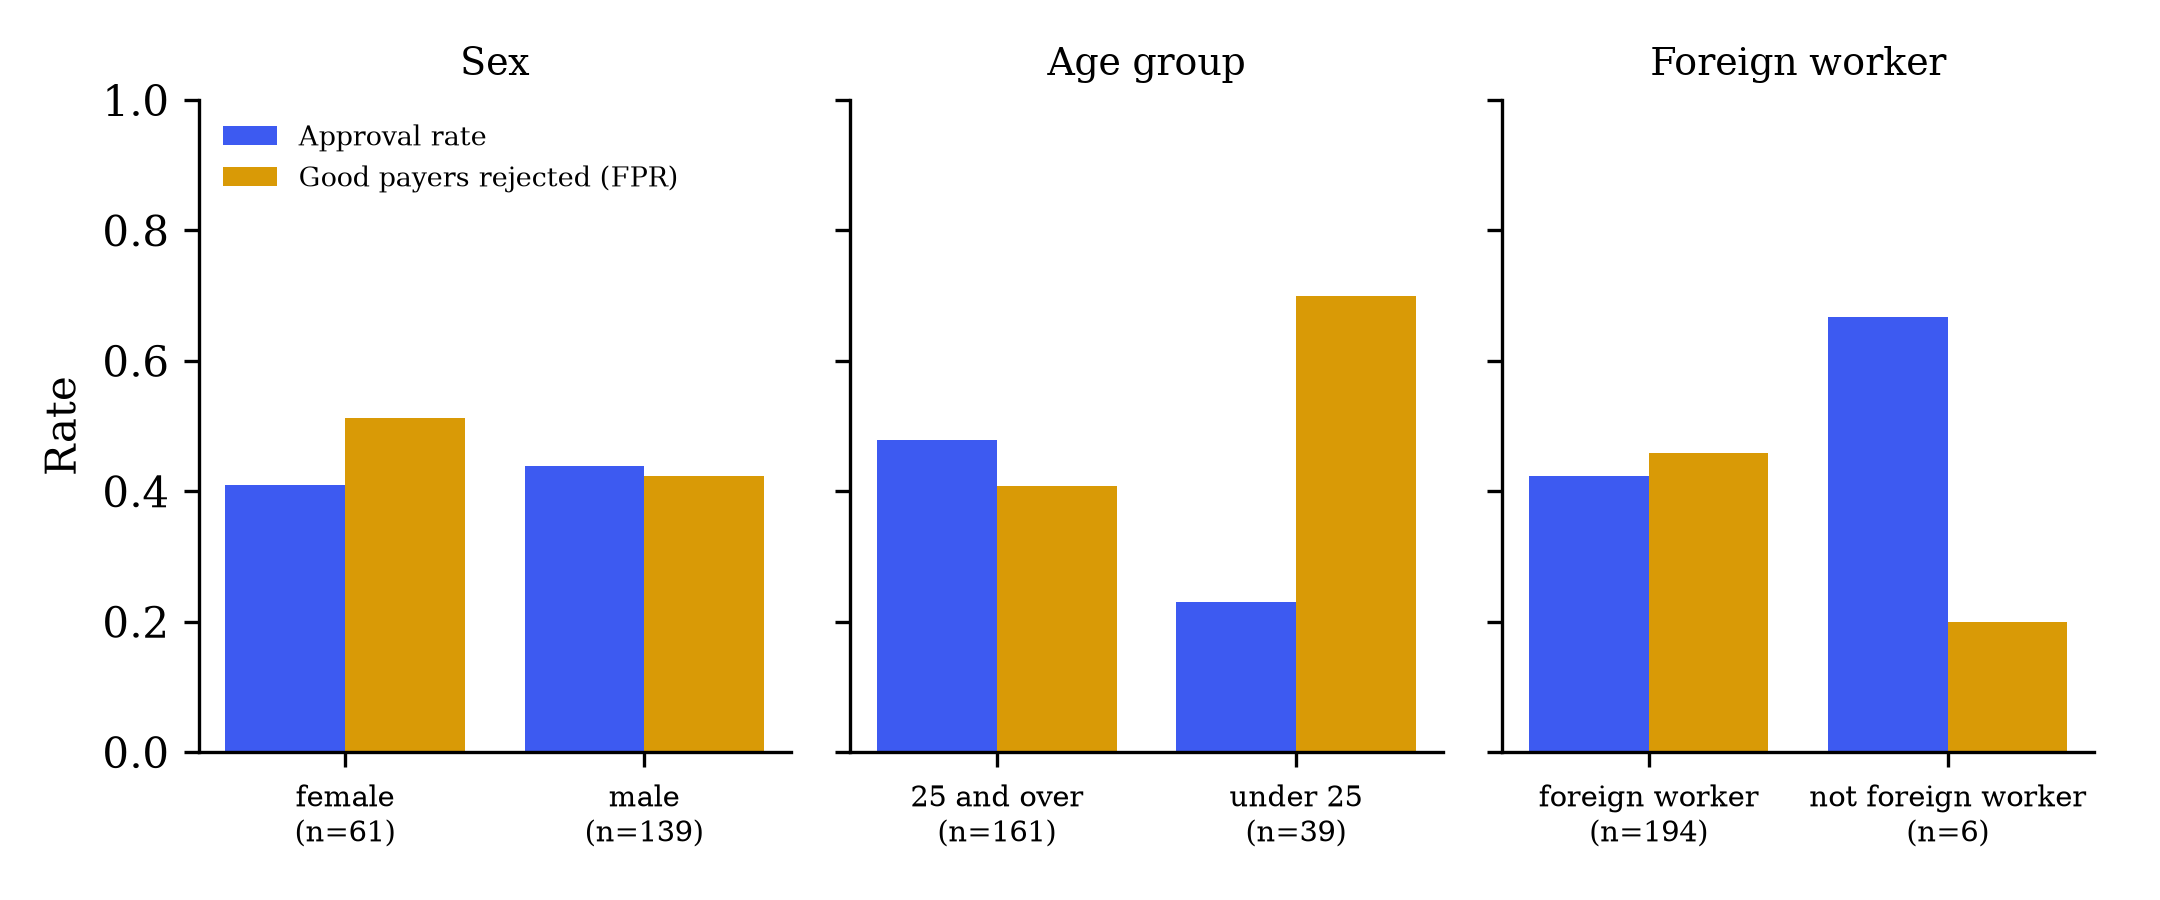
\includegraphics[width=0.95\textwidth,height=\textheight]{figures/fairness_groups.png}
\caption{Approval rate and false-positive rate by group on the
test set.}
\end{figure}

\textbf{Age.} Applicants under 25 are approved at roughly half the rate
of older applicants (23.1\% vs 47.8\%), and creditworthy young
applicants are wrongly flagged 70.0\% of the time, against 40.8\% for
older applicants. Part of the approval gap reflects the data: only
51.3\% of young test applicants were actually good, against 74.5\% of
older ones. Age is also a direct model input, although its global SHAP
importance is moderate. The disparity in false-positive rates goes
beyond the difference in base rates and is the most important fairness
finding of this study.

\textbf{Sex.} Approval rates are similar (41.0\% vs 43.9\%; DPD 0.029),
so demographic parity is nearly satisfied. Error rates are not:
creditworthy women are wrongly rejected more often than creditworthy men
(51.2\% vs 42.4\%), and women who default are missed more often (25.0\%
vs 10.0\%). Sex is not a model input, so these differences arise through
correlated features, illustrating that excluding a protected attribute
does not guarantee equal treatment {[}8{]}. With 61 women in the test
set, these rates are imprecise.

\textbf{Foreign-worker status.} Only 6 test applicants are not foreign
workers, so the computed gap (DPD 0.244) is statistically meaningless; a
single different decision would change the group's approval rate by
about 17 percentage points. We report the result for completeness and
explicitly mark it as unreliable.

These results show that the auditing component works as intended: it
surfaces disparities that would remain invisible from aggregate metrics.
They do not show that the model is fair, and they do not establish the
causes of the disparities.

\hypertarget{discussion}{%
\section{19. Discussion}\label{discussion}}

\textbf{RQ1 (prediction).} All three classifiers reached a test ROC-AUC
of about 0.81, and the cross-validated differences were below 0.025. On
a dataset of 1,000 applicants, the choice among reasonable models
matters far less than the decision threshold, which moved recall from
0.35 to 0.85. This is consistent with benchmark studies reporting modest
gaps between well-tuned methods {[}1{]}, {[}2{]}.

\textbf{RQ2 (explanation).} SHAP produced explanations that are
consistent with credit-domain intuition: liquidity indicators (checking
and savings balances), loan duration and repayment history dominate.
Summing one-hot contributions back to original attributes made
explanations readable by non-specialists, and the additivity check
ensures each explanation accounts for the predicted probability.
Nevertheless, SHAP explains the model rather than the world; for
instance, the finding that applicants with \emph{no} checking account
appear lower-risk than those with a small balance reflects a pattern in
this historical sample, not a causal effect.

\textbf{RQ3 (fairness).} The audit identified a substantial age
disparity and unequal error rates by sex despite near-equal approval
rates. It also showed that one of the three groupings cannot be assessed
reliably with this dataset. As established in {[}21{]}, {[}22{]}, when
base rates differ (here 51\% vs 75\% good by age), equal approval rates,
equal error rates and calibration cannot all hold, so mitigation would
require an explicit choice of fairness criterion.

\textbf{RQ4 (stability).} Decisions were stable for 96.5\% of test
applicants under ±5\% changes to amount and duration, and all
instability was concentrated near the threshold. The MEDIUM risk band
therefore serves a practical purpose by highlighting cases where an
automated decision is least reliable.

\textbf{RQ5 (integration).} The prototype demonstrates that the four
analyses can be served together through one API with a consistent
schema, without compromising the evaluation protocol: model selection,
threshold search and preprocessing all use training data only, and the
test set is used solely for reporting.

\hypertarget{limitations}{%
\section{20. Limitations}\label{limitations}}

\begin{itemize}
\tightlist
\item
  \textbf{Dataset size.} 1,000 applicants and a 200-applicant test set
  give wide uncertainty on every metric, especially group-level rates.
  No confidence intervals are reported yet.
\item
  \textbf{Dataset age and context.} The data come from a single German
  bank, with amounts in Deutsche Mark, and were published in 1994.
  Neither the population nor the lending practices are representative of
  contemporary markets, including the Indian context.
\item
  \textbf{Data quality.} Grömping {[}16{]} documented coding errors in
  the original attribute descriptions. We used the original, widely
  cited version, so some attribute meanings may be inaccurate.
\item
  \textbf{Sensitive attributes.} Sex is derived from a combined
  marital-status field without a ``single female'' category; only 37
  applicants (6 in the test set) are not foreign workers. No information
  on other protected characteristics is available.
\item
  \textbf{Fairness metrics.} The status thresholds (0.10 / 0.20) are
  heuristics. Group metrics do not capture individual fairness or the
  causes of disparity, and different fairness definitions can conflict.
\item
  \textbf{Explanation reliability.} SHAP values depend on the background
  sample and on the interventional assumption, and post-hoc explanations
  can be unstable or manipulable {[}10{]}, {[}11{]}.
\item
  \textbf{Stability test scope.} Only two continuous features are
  randomly perturbed, at a single noise level; this is not a formal
  robustness guarantee.
\item
  \textbf{Calibration.} Predicted probabilities have not been
  calibrated, so a reported ``41\% probability of default'' should be
  read as a model score rather than an exact frequency.
\item
  \textbf{No real-world validation.} The system has not been evaluated
  with lenders, credit officers or applicants, and it includes no
  authentication or persistent storage. It is not suitable for real
  lending decisions.
\end{itemize}

\hypertarget{current-research-progress-approximately-70-of-the-research-objective}{%
\section{21. Current Research Progress (Approximately 70\% of the
Research
Objective)}\label{current-research-progress-approximately-70-of-the-research-objective}}

Table VIII summarises the status of each sub-objective defined in
Section 3.

\textbf{Table VIII. Progress against research objectives}

\begin{longtable}[]{@{}
  >{\raggedright\arraybackslash}p{(\columnwidth - 4\tabcolsep) * \real{0.3333}}
  >{\raggedright\arraybackslash}p{(\columnwidth - 4\tabcolsep) * \real{0.3333}}
  >{\raggedright\arraybackslash}p{(\columnwidth - 4\tabcolsep) * \real{0.3333}}@{}}
\toprule\noalign{}
\begin{minipage}[b]{\linewidth}\raggedright
Objective
\end{minipage} & \begin{minipage}[b]{\linewidth}\raggedright
Status
\end{minipage} & \begin{minipage}[b]{\linewidth}\raggedright
Evidence
\end{minipage} \\
\midrule\noalign{}
\endhead
\bottomrule\noalign{}
\endlastfoot
O1 Prediction: three models, CV tuning, held-out metrics & Completed &
Table I, Table II, saved training metadata \\
O2 Cost-aware threshold from training data & Completed & Threshold 0.27,
cost reduced from 203 to 108 \\
O3 Local and global SHAP explanations & Completed & Fig. 4, Table IV,
additivity test \\
O4 Fairness audit with sample-size caveats & Completed (audit);
mitigation not started & Tables VI--VII, Fig. 5 \\
O5 Stability analysis & Partially completed & Table V; limited to two
perturbed features and one noise level \\
O6 Integrated API and dashboard & Completed (prototype) & FastAPI
service, React dashboard \\
Software quality and documentation & Completed & 19 backend + 8 frontend
tests, README, methodology notes, notebook \\
Statistical uncertainty (confidence intervals) & Not started & --- \\
Fairness mitigation and comparison & Not started & --- \\
External validation on additional data & Not started & --- \\
User evaluation of explanations & Not started & --- \\
\end{longtable}

The core pipeline (prediction, explanation, fairness auditing, stability
testing and their integration) is implemented and evaluated, which we
estimate as approximately 70\% of the research objective. The remaining
30\% concerns the depth and validity of the findings rather than
additional features:

\begin{enumerate}
\def\labelenumi{\arabic{enumi}.}
\tightlist
\item
  bootstrap confidence intervals for all model and group metrics;
\item
  at least one fairness-mitigation method (for example Fairlearn's
  threshold optimiser or exponentiated-gradient reduction {[}23{]}),
  compared before and after on accuracy, cost and fairness;
\item
  probability calibration and its effect on the cost-optimal threshold;
\item
  an extended stability study covering more features, several noise
  levels and the stability of SHAP explanations themselves;
\item
  validation on the corrected South German Credit data {[}16{]} and, if
  possible, a larger contemporary dataset;
\item
  a small user study assessing whether the explanations are
  understandable to non-technical users.
\end{enumerate}

\hypertarget{conclusion}{%
\section{22. Conclusion}\label{conclusion}}

This paper presented a working prototype that treats a credit decision
as more than a label. For every applicant, the system returns a
cost-aware risk decision, a SHAP explanation in terms of the original
attributes and a stability check; at the model level, it reports
evaluation metrics and a group-fairness audit. On the German Credit
dataset, a random forest selected through cross-validation reached a
test ROC-AUC of 0.809 and, with a threshold derived from the dataset's
5:1 cost matrix, identified 85\% of defaulters. Explanations highlighted
liquidity, loan duration and credit history as the main drivers. The
fairness audit revealed a pronounced age disparity and unequal error
rates by sex, and the stability analysis showed that decisions change
only for applicants near the threshold. The prototype is not a
production lending system, and its fairness findings are evidence of
disparities to be addressed, not proof of a fair model. Its main value
is to show, in an open and reproducible way, how transparency, fairness
checking and robustness testing can accompany every prediction.

\hypertarget{future-work}{%
\section{23. Future Work}\label{future-work}}

Beyond the remaining items listed in Section 21, future work could:

\begin{itemize}
\tightlist
\item
  compare post-hoc explanations with inherently interpretable models
  such as monotonic gradient boosting or generalised additive models,
  following the argument in {[}4{]};
\item
  add counterfactual explanations (``what change would lead to
  approval?'') to support applicants;
\item
  study the interaction between threshold choice and group fairness;
\item
  add authentication, persistent auditable storage and monitoring for
  data drift if the system were moved towards deployment.
\end{itemize}

\hypertarget{references}{%
\section{References}\label{references}}

{[}1{]} B. Baesens, T. Van Gestel, S. Viaene, M. Stepanova, J. Suykens,
and J. Vanthienen, ``Benchmarking state-of-the-art classification
algorithms for credit scoring,'' \emph{Journal of the Operational
Research Society}, vol.~54, no. 6, pp.~627--635, 2003, doi:
10.1057/palgrave.jors.2601545.

{[}2{]} S. Lessmann, B. Baesens, H.-V. Seow, and L. C. Thomas,
``Benchmarking state-of-the-art classification algorithms for credit
scoring: An update of research,'' \emph{European Journal of Operational
Research}, vol.~247, no. 1, pp.~124--136, 2015, doi:
10.1016/j.ejor.2015.05.030.

{[}3{]} X. Dastile, T. Celik, and M. Potsane, ``Statistical and machine
learning models in credit scoring: A systematic literature survey,''
\emph{Applied Soft Computing}, vol.~91, Art. no. 106263, 2020, doi:
10.1016/j.asoc.2020.106263.

{[}4{]} C. Rudin, ``Stop explaining black box machine learning models
for high stakes decisions and use interpretable models instead,''
\emph{Nature Machine Intelligence}, vol.~1, no. 5, pp.~206--215, 2019,
doi: 10.1038/s42256-019-0048-x.

{[}5{]} M. T. Ribeiro, S. Singh, and C. Guestrin, ``\,`Why should I
trust you?': Explaining the predictions of any classifier,'' in
\emph{Proc. 22nd ACM SIGKDD Int. Conf. Knowledge Discovery and Data
Mining}, 2016, pp.~1135--1144, doi: 10.1145/2939672.2939778.

{[}6{]} S. M. Lundberg and S.-I. Lee, ``A unified approach to
interpreting model predictions,'' in \emph{Advances in Neural
Information Processing Systems 30 (NIPS 2017)}, 2017, pp.~4765--4774.

{[}7{]} N. Mehrabi, F. Morstatter, N. Saxena, K. Lerman, and A.
Galstyan, ``A survey on bias and fairness in machine learning,''
\emph{ACM Computing Surveys}, vol.~54, no. 6, Art. no. 115, 2021, doi:
10.1145/3457607.

{[}8{]} S. Barocas, M. Hardt, and A. Narayanan, \emph{Fairness and
Machine Learning: Limitations and Opportunities}. Cambridge, MA, USA:
MIT Press, 2023.

{[}9{]} A. Fuster, P. Goldsmith-Pinkham, T. Ramadorai, and A. Walther,
``Predictably unequal? The effects of machine learning on credit
markets,'' \emph{The Journal of Finance}, vol.~77, no. 1, pp.~5--47,
2022, doi: 10.1111/jofi.13090.

{[}10{]} D. Alvarez-Melis and T. S. Jaakkola, ``On the robustness of
interpretability methods,'' arXiv preprint arXiv:1806.08049, 2018.

{[}11{]} D. Slack, S. Hilgard, E. Jia, S. Singh, and H. Lakkaraju,
``Fooling LIME and SHAP: Adversarial attacks on post hoc explanation
methods,'' in \emph{Proc. AAAI/ACM Conf. AI, Ethics, and Society (AIES
'20)}, 2020, pp.~180--186, doi: 10.1145/3375627.3375830.

{[}12{]} L. Breiman, ``Random forests,'' \emph{Machine Learning},
vol.~45, no. 1, pp.~5--32, 2001, doi: 10.1023/A:1010933404324.

{[}13{]} T. Chen and C. Guestrin, ``XGBoost: A scalable tree boosting
system,'' in \emph{Proc. 22nd ACM SIGKDD Int. Conf. Knowledge Discovery
and Data Mining}, 2016, pp.~785--794, doi: 10.1145/2939672.2939785.

{[}14{]} H. Hofmann, ``Statlog (German Credit Data),'' UCI Machine
Learning Repository, 1994. {[}Online{]}. Available:
https://doi.org/10.24432/C5NC77

{[}15{]} F. Kamiran and T. Calders, ``Data preprocessing techniques for
classification without discrimination,'' \emph{Knowledge and Information
Systems}, vol.~33, no. 1, pp.~1--33, 2012, doi:
10.1007/s10115-011-0463-8.

{[}16{]} U. Grömping, ``South German Credit,'' UCI Machine Learning
Repository, 2019. {[}Online{]}. Available:
https://archive.ics.uci.edu/dataset/573

{[}17{]} F. Doshi-Velez and B. Kim, ``Towards a rigorous science of
interpretable machine learning,'' arXiv preprint arXiv:1702.08608, 2017.

{[}18{]} S. M. Lundberg, G. Erion, H. Chen, A. DeGrave, J. M. Prutkin,
B. Nair, R. Katz, J. Himmelfarb, N. Bansal, and S.-I. Lee, ``From local
explanations to global understanding with explainable AI for trees,''
\emph{Nature Machine Intelligence}, vol.~2, no. 1, pp.~56--67, 2020,
doi: 10.1038/s42256-019-0138-9.

{[}19{]} N. Bussmann, P. Giudici, D. Marinelli, and J. Papenbrock,
``Explainable machine learning in credit risk management,''
\emph{Computational Economics}, vol.~57, no. 1, pp.~203--216, 2021, doi:
10.1007/s10614-020-10042-0.

{[}20{]} M. Hardt, E. Price, and N. Srebro, ``Equality of opportunity in
supervised learning,'' in \emph{Advances in Neural Information
Processing Systems 29 (NIPS 2016)}, 2016, pp.~3315--3323.

{[}21{]} J. Kleinberg, S. Mullainathan, and M. Raghavan, ``Inherent
trade-offs in the fair determination of risk scores,'' in \emph{Proc.
8th Innovations in Theoretical Computer Science Conf. (ITCS 2017)},
LIPIcs vol.~67, 2017, pp.~43:1--43:23, doi: 10.4230/LIPIcs.ITCS.2017.43.

{[}22{]} A. Chouldechova, ``Fair prediction with disparate impact: A
study of bias in recidivism prediction instruments,'' \emph{Big Data},
vol.~5, no. 2, pp.~153--163, 2017, doi: 10.1089/big.2016.0047.

{[}23{]} H. Weerts, M. Dudík, R. Edgar, A. Jalali, R. Lutz, and M.
Madaio, ``Fairlearn: Assessing and improving fairness of AI systems,''
\emph{Journal of Machine Learning Research}, vol.~24, no. 257, pp.~1--8,
2023.

{[}24{]} I. J. Goodfellow, J. Shlens, and C. Szegedy, ``Explaining and
harnessing adversarial examples,'' in \emph{Proc. 3rd Int. Conf.
Learning Representations (ICLR)}, 2015, arXiv:1412.6572.

{[}25{]} F. Pedregosa \emph{et al.}, ``Scikit-learn: Machine learning in
Python,'' \emph{Journal of Machine Learning Research}, vol.~12,
pp.~2825--2830, 2011.

{[}26{]} T. Fawcett, ``An introduction to ROC analysis,'' \emph{Pattern
Recognition Letters}, vol.~27, no. 8, pp.~861--874, 2006, doi:
10.1016/j.patrec.2005.10.010.

{[}27{]} C. Elkan, ``The foundations of cost-sensitive learning,'' in
\emph{Proc. 17th Int. Joint Conf. Artificial Intelligence (IJCAI)},
2001, pp.~973--978.

\end{document}
